% \documentclass[11pt,phdthesis,oneside]{cssethesis}
\documentclass{svmult}
%1234567890123456789012345678901234567890123456789012345678901234567890123456789

% per springer/quickstart.pdf
\usepackage{mathptmx,helvet,courier,makeidx,multicol,footmisc}
\usepackage{amsfonts,ifthen,color}
\usepackage{natbib}
\usepackage{times,setspace}

\usepackage{natbib,verbatim}
% \usepackage{pdflscape}
\usepackage{amssymb,latexsym,amsmath}
\usepackage{graphicx}
\usepackage[table, xcdraw]{xcolor}
\usepackage{lscape}
\usepackage{algorithm, algpseudocode}
\usepackage{url}
\usepackage{mathtools}


\newcommand{\deltap}{\ensuremath{\Delta P}}
\newcommand{\intinf}{\ensuremath{\int_{-\infty}^{\infty}}}
\newcommand{\summ}{\ensuremath{\sum_{i=1}^m}}
\newcommand{\summj}{\ensuremath{\sum_{j=1}^m}}
\newcommand{\ddpi}[1]{\ensuremath{\frac{\delta {#1}}{\delta p_i}}}
\newcommand{\DDpi}[1]{\ensuremath{\frac{\delta^2 {#1}}{\delta p_i^2}}}
\newcommand{\Ddpidpj}[1]{\ensuremath{\frac{\delta^2 {#1}}{\delta p_i \delta p_j}}}

\newcommand{\kl}{\ensuremath{\mathrm{kl}}}
\newcommand{\AL}{\ensuremath{\mathrm{AL}}}
\newcommand{\IR}[1]{\ensuremath{\mathrm{IR}_{#1}}}
\newcommand{\BIR}{\ensuremath{\mathrm{BIR}}}
\newcommand{\IROLD}{\IR{\textit{old}}}
\newcommand{\IRG}{\IR{G}}
\newcommand{\prior}{\ensuremath{\phi}}
\newcommand{\ssec}[1]{\S{}\ref{#1}}

\renewcommand{\cite}{\citep}

\hyphenation{pre-ce-dence Final-ly}

%%%%%%%%%%%%%%%
% 1. Commands
%%%%%%%%%%%%%%%
\newcommand{\dsp}{\setlength{\baselineskip}{24truept}}  %double spacing
\newcommand{\ssp}{\setlength{\baselineskip}{13.6truept}}%single spacing
\newcommand{\hs}{\hspace{0.2in}}
\newcommand{\vs}{\vspace{-0.5in}}
\newcommand{\be}{\begin{equation}}
\newcommand{\ee}{\end{equation}}
\newcommand{\bd}{\begin{description}}
\newcommand{\ed}{\end{description}}
\newcommand{\ben}{\begin{enumerate}}
\newcommand{\een}{\end{enumerate}}
\newcommand{\beq}{\begin{quote}}
\newcommand{\eeq}{\end{quote}}
\newcommand{\bi}{\begin{itemize}}
\newcommand{\ei}{\end{itemize}}
\newcommand{\bea}{\begin{eqnarray}}
\newcommand{\eea}{\end{eqnarray}}
\newcommand{\bua}{\begin{eqnarray*}}
\newcommand{\eua}{\end{eqnarray*}}
\newcommand{\ov}[1]{\overline{#1}}
\newcommand{\ul}[1]{\underline{#1}}
\newcommand{\ba}{\begin{array}}
\newcommand{\ea}{\end{array}}
\newcommand{\bfig}{\begin{figure}}
\newcommand{\efig}{\end{figure}}
\newcommand{\bc}{\begin{center}}
\newcommand{\ec}{\end{center}}
\newcommand{\bt}{\begin{table}}
\newcommand{\et}{\end{table}}
\newcommand{\btab}{\begin{tabular}}
\newcommand{\etab}{\end{tabular}}

\newcommand{\Rarr}{\ensuremath{\Rightarrow}}
\newcommand{\rarr}{\ensuremath{\rightarrow}}
\newcommand{\Larr}{\ensuremath{\Leftarrow}}
\newcommand{\larr}{\ensuremath{\leftarrow}}
\newcommand{\lrarr}{\ensuremath{\leftrightarrow}}
\newcommand{\LRarr}{\ensuremath{\LeftRightArrow}}
\newcommand{\rl}{\ensuremath{\rightleftharpoons}}
\renewcommand{\tilde}{\~{\ }\hspace*{-.7ex}}
\newcommand{\abs}[1]{\ensuremath{~|{#1}|~}}
\newcommand{\seq}[1]{\langle\mbox{#1}\rangle}

\renewcommand{\vec}[1]{\hat{\mathbf{#1}}}  % normal \vec not working

\newcommand{\boxup}[1]
{\beq
\fbox{
\parbox{2in}{#1}}
\eeq
}

\newcommand{\myitem}{\vspace*{-0.5ex} \item }

%\newcounter{modulenum}
%\setcounter{modulenum}{1}
%\newcommand{\module}{% Define module
%\section*{Module \arabic{modulenum}~}
%\addtocounter{modulenum}{1}
%}
%
%\newcounter{problemnum}
%\setcounter{problemnum}{1}
%\newcommand{\problem}{% Define problem
%\subsubsection*{Problem \arabic{problemnum}~}
%\addtocounter{problemnum}{1}
%}
%
%\newcounter{examplenum}
%\setcounter{examplenum}{1}
%\newcommand{\example}{% Define example
%\subsubsection*{Example \arabic{examplenum}~}
%\addtocounter{examplenum}{1}
%}

\newcommand{\mc}[1]{\ensuremath{\mathcal{#1}}}
\newcommand{\optional}[1]{\textcolor{blue}{#1}}
\newcommand{\mmlcpt}{$mbMML_{CPT}$ }
\newcommand{\mbptmml}{$MBPT_{mml}$ }
\DeclareMathOperator*{\argmin}{arg\,min}
\DeclarePairedDelimiter\floor{\lfloor}{\rfloor}
\newcommand{\qedwhite}{\hfill \ensuremath{\Box}}


\newcommand{\indep}{~\raisebox{-0.3ex}{\rotatebox{90}{\ensuremath{\models}}}}
\newcommand{\dep}{\not \hspace*{-1.2ex}\indep}
%\newcommand{\textunder}[1]{$_{\text{#1}}$}

%%%%%%%%%%%%%%%%%%%%%%%%%%%%%%
% 2. Theorems & Environments
%%%%%%%%%%%%%%%%%%%%%%%%%%%%%%

\newtheorem{fact}{Fact}
\newtheorem{hyp}{Hypothesis}
\newtheorem{lemm}{Lemma}
%\newtheorem{exercise}{Exercise}
\newtheorem{Example}{Example}
\newtheorem{prop}{Property}
\newtheorem{defn}{Definition}
\newtheorem{result}{Result}
\newtheorem{conject}{Conjecture}
\newtheorem{princ}{Principle}

%\newenvironment{proof}[1]{{\bf #1}\em}{\/}
\newenvironment{prf}{\rm}{}

  


%%%%%%%%%%
% Misc.
%%%%%%%%%%


%%%%%%%%%%
% Misc.
%%%%%%%%%%

\renewcommand{\floatpagefraction}{0.7}

\newcommand{\cs}[1]{\mbox{c}_{#1}}
\newcommand{\sn}[1]{\mbox{s}_{#1}}
\newcommand{\threevec}[3]{
        \left[ 
        \begin{array}{c} #1 \\ #2 \\ #3 \end{array}
        \right]
}
\newcommand{\hvec}[4]{
        \left[ 
        \begin{array}{c} #1 \\ #2 \\ #3 \\ #4 \end{array}
        \right]
}
\newcommand{\qvec}[1]{
        \left[
        \begin{array}{c} 0 \\ #1 \end{array}
        \right]
}

\newcommand{\newspecial}[1]{
        \ifnum\includefigs>0
                \special{#1}
        \fi
}

\newcommand{\slidehead}[2][2ex]{%
  \slideheading{#2}\vspace{#1}
  \small
  }

\newcommand{\sh}[1]{\slideheading{#1}}

\newcommand{\subheader}[3]{\vspace{#1}\bc{\em #3}\ec\vspace{#2}}

\def\makeslideheading#1{%
  \begin{center}\Large\bf #1\end{center}}

\newboolean{draftp}

\newcommand{\new}[1]{
\textcolor{red}{#1}
}
\newcommand{\newcomment}[1]{
\ifthenelse{\boolean{draftp}}{#1}{}
}


%%%%%%%%%%%%%%%%%%%%
% 3. Page setup
%%%%%%%%%%%%%%%%%%%%


%\setlength{\parindent}{0cm}

\newcommand{\standardpagesetup}{

\addtolength{\textheight}{55mm}
\addtolength{\textwidth}{25mm}
\addtolength{\voffset}{-31mm}
\addtolength{\marginparwidth}{30mm}
%\setlength{\columnsep}{25mm}
%\setlength{\columnseprule}{0.5pt}
\oddsidemargin = 0 mm
\topmargin = 0 mm

%\textwidth = 156 mm
%\textheight = 243 mm
%\parindent = 6 mm
\parskip = 2 mm
\textfloatsep = 0 mm
\intextsep = 0 mm

  }
\newcommand{\pdfpagesetup}{

\addtolength{\textheight}{40mm}
\addtolength{\textwidth}{25mm}
\addtolength{\voffset}{-31mm}
\addtolength{\marginparwidth}{30mm}
%\setlength{\columnsep}{25mm}
%\setlength{\columnseprule}{0.5pt}
\oddsidemargin = 0 mm
\topmargin = 20 mm

%\textwidth = 156 mm
%\textheight = 243 mm
\parindent = 6 mm
%\parskip = 0 mm
\textfloatsep = 0 mm
\intextsep = 0 mm

  }


% afour (a4)
% Hopefully the a4paper option does these, but for reference:
\newcommand{\afour}{
  \paperheight 297mm
  \paperwidth  210mm
  \textheight  247mm % Pageheight - 50mm
  \textwidth   160mm % Pagewidth - 50mm
  \oddsidemargin -5mm
  \topmargin     -15mm
%  \slideheight 152mm % For seminar.sty. As per manual. But use sem-a4.sty.
%  \slidewidth  222mm % Likewise.
  }

% Also try a4 dimensions of 167 and 225 for slideheight/width.


%%%%%%%%%%%%%%%%%%
% 4. Natbib Cites
%%%%%%%%%%%%%%%%%%

%\bibpunct[, ]{(}{)}{,}{a}{,}{,}


%\makeindex

%%%%%%%%%%%%%%%%%%%%%%%%%%%%%%%%%%%%%%%%%%%%%%%%%%%%%%%%%%%%%%%%%%%%%%%%%%%%%%%%
%1234567890123456789012345678901234567890123456789012345f678901234567890123456789

\begin{document}


%%%%%%%%%%%%%%%%%%%%%%%%%%%%%%%%%%%%%%%%%%%%%%%%%%%%%%%%%%%%%%%%%%%%%%%%%%%%%%%%

\title*{Markov Blanket Discovery using Minimum Message Length}
%\subtitle{Do you have a subtitle?\\ If so, write it here}

%\titlerunning{Short form of title}        % if too long for running head

\author{Yang Li         \and
        Kevin B Korb  \and
        Lloyd Allison
}

%\authorrunning{Short form of author list} % if too long for running head
\iffalse
\institute{F. Author \at
              first address \\
              Tel.: +123-45-678910\\
              Fax: +123-45-678910\\
              \email{fauthor@example.com}           %  \\
%             \emph{Present address:} of F. Author  %  if needed
           \and
           S. Author \at
              second address
}
\fi
\date{Received: date / Accepted: date}
% The correct dates will be entered by the editor

\maketitle

\abstract{Causal discovery automates the learning of causal Bayesian
  networks from data and has been of active interest from their
  beginning. With the sourcing of large datasets off the internet,
  interest in scaling up to very large datasets has grown. One
  approach to this is to parallelize search using Markov Blanket (MB)
  discovery as a first step in learning a full causal model, followed
  by a process of combining MBs in a global causal model. We develop
  and explore three new methods of MB discovery using Minimum Message
  Length (MML) scoring and compare them empirically to the best
  existing methods, whether developed specifically as MB discovery or
  as feature selection (which can be understood as equivalent to MB
  discovery).  Our best MML method is consistently competitive and has
  some advantageous features.}

\keywords{Markov Blanket, feature selection, causal discovery, Bayesian network, Minimum Message Length}

\section{Introduction}
\label{sec:intro}
The assumptions made throughout this paper (some of these are made by the MML principle):
\begin{enumerate}
\item The dataset is complete, with no hidden variables, discrete and \textit{i.i.d.}. 
\item The parameters are independent and follow symmetric Dirichlet distributions. 
\end{enumerate} 

{\em Terminology.} In the causal discovery and
Bayesian network literature, ``local structure'' refers to any
dependencies between the parameters within the conditional
probabiility distribution associated with a particular
variable. Therefore, we shall use ``regiional structure'' to refer to
the causal structure within the Markov Blanket of a variable (i.e.,
its graphical structure), to contrast it both with this local
structure and with the global causal structure represented by the
entire Bayesian network.

and local model refer to structure within a CPT. We may need to change the term to substructure or something.
%\iffalse
\begin{itemize}
\item identify gap
\item why use mml, it has been shown to provide a robust induction method in various domains, cite camml
\end{itemize}

The structure of a Bayesian network (BN) is a directed acyclic graph (DAG) where each node represents a variable and each arc $X \to Y$ represents a direct causal relationship with $X$ being the cause of $Y$. Causal model structures can be built based on expert knowledge, then interrogated and validated in real world scenarios. Nevertheless, the lack of expertise and the complexity of manually building large models motivate automated learning. 

Causal discovery refers to an algorithm-based process of reconstructing generating causal structures from observational data. Due to the NP-hardness of this problem\cite{chickering1995learning}, heuristics are often used to find approximate solutions on large datasets. An alternative is the local-to-global (LGL) paradigm that finds local structures within subsets of variables then unifies them into a global structure. One choice of a variable subset is the minimal subset of all variables $V$ that satisfies  
\begin{align*}
X \indep V \setminus \{X, MB(X)\} \mid MB(X).
\end{align*}
It is known as the Markov Blanket \cite{pearl1988probabilistic}of the variable $X$, denoted by $MB(X)$. It is built upon the Markov property of a Bayesian network, which states that the non-descendants of a variable $X$ are conditionally independent of $X$ given its parent variables. 

\textcolor{red}{Markov Blanket is also known as Markov boundary in some literatures, such as Acid 2013}. 

Section 2, 3 and 4 focus on learning the Markov Blanket of a variable using the minimum message length principle. Once the Markov Blankets are learned, these subsets of variables are built into local polytrees (section 5), whose space is much smaller than the space of DAGs. Some initial works of the globalised step are briefly mentioned in section 6 and 7.  

Almost all works on metric-based approach learn the local structure around a target and in consequence identify the Markov Blanket of it. We believe Markov Blanket learning can be separated from local structure learning, and hence has a potential to reduce the time complexity and increase the robustness of a learner regarding small samples. In the next section, we briefly introduce the MML principle and its exact formula used for our \mmlcpt algorithm.

Almost all LGL algorithms focus on exploring undirected local skeletons then merging them into one graph so that arcs can be directed using heuristics. We believe there are a decent number of overlapping arcs that need not to be learned in all neighboring local structure, but will be covered after the local-to-global process. Motivated by this, we proposed to restrict local DAGs within MBs to polytrees that are induced subgraphs of DAGs but less dense. In addition, we proved that the total number of restricted Markov Blanket polytrees (MBPTs) is sub-exponential, hence the optimal MBPT in terms of a decomposable score can be efficiently searched for small and medium MBs. The paper is structured as the following. Section 2 briefly introduced a MB discovery algorithm called $mbMML_{CPT}$ that we developed and is currently under review.  In section 3.1, we derived a formula for counting all MBPTs and stated an algorithm for enumerating them. Section 3.2 outlined our $mml_{MBPT}$ algorithm for learning causal model. In section 4, our algorithm was empirically compared with several other causal learners on real models.  

The paper is organised as following. Section presented related works in Markov Blanket discovery. Section 3 introduced details about MML and how it was used as an objective function in \mmlcpt. Section 4 contains the experiments on comparing \mmlcpt with several state-of-the-art Markov Blanket discovery algorithms using both artificial and real world models. 
%\fi 

\section{Related work} 
\label{sec:related}
The concept of a Markov Blanket (MB) of a (target) variable is the
smallest subset of variables conditioning on which the target is
independent of the remaining variables of a
model.\footnote{Originally, this is how \citet{pearl1988probabilistic}
  defined ``Markov boundaries'', but the literature has migrated
  ``Markov blankets'' to this minimalist sense.}  This implies that
other variables beyond the blanket carry no additional information
about the target, i.e., that Markov Blankets are the optimal feature
subsets for prediction
\citep{koller1996toward,cooper1997evaluation,cheng2001kdd}. In a
Bayesian network a variable's MB contains its parents and children and
its spouses (i.e., the children's other parents, see
Figure~\ref{fg:MB}).

\begin{figure}[htb]
  \centering
    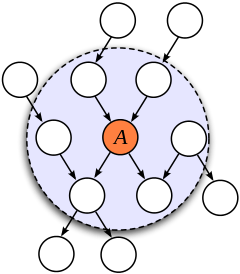
\includegraphics[scale=0.6]{figures/MB.png}
  \caption{Markov Blanket for $A$ in a dag.}
  \label{fg:MB}
\end{figure}

A Bayesian network with $n$ variables can be viewed as a union of its $n$ 
distinct Markov Blankets. It follows that one approach to reducing the
complexity of learning a full causal Bayesian network is to learn the
structures of $n$  MBs independently and then stitch them together. A
good review of this approach is \citet{aliferis2010localb}.

%Although Markov Blankets are proper subsets of a domain, finding the right candidates is not much easier than learning a Bayesian network over the domain.

A natural way of doing this is suggested by the conditional
independence definition of Markov Blankets: testing dependencies
between a target and everything else given each possible subset of
other variables, looking for the minimal subsets yielding zero
dependency. An exhaustive search of this kind would, of course, be
exponential in the size of the network. But we can try a heuristic,
instead of exhaustive, search. This was done by
\citet{margaritis1999bayesian}. Their work laid the foundation for a
constraint-based Markov Blanket discovery that typically consists of
alternating addition and deletion
phases. \citet{tsamardinos2003algorithms} improved on this work by
adding those variables to the candidate MB having the strongest
dependencies with the target in advance. While employing the same
statistical tests and heuristics, another algorithm that learns the
direct neighbors and spouses separately has proven superior, and hence
has been widely adopted in later constraint-based methods (see
\citet{aliferis2003hiton,tsamardinos2003time,pena2007towards,fu2008fast,aliferis2010locala,demorais2010novel,liu2016swamping}). In
particular, this improved strategy looks at the dependencies with the
target at a distance of one and two neighbors separately.  Neighbors
two removed are then filtered to remove false positives. At the end of
each learning process, the discovered MB are then required
to satisfy the symmetry condition for Markov Blankets (Proposition
\ref{prop:sym} in Section \ref{sec:mb}), which further helps to
identify false positives.

Metric-based learners, having proven themselves highly effective in
causal discovery, have subsequently been applied to Markov Blanket
discovery. In contrast to metric learning of full Bayesian networks,
the search space is restricted to local (sub-) structures around a
target variable without regard for unrelated adjacencies
\citep{cooper1997evaluation,madden2002new,acid2013score}. Given that
most real models are sparse, Markov Blankets tend to be small. This
allows exact algorithms for learning small Bayesian networks to be
applied to find optimal local structures
independently. \citet{niinimaki2012local} published the first exact
Markov Blanket learning algorithm and also applied it to scale up to
exact general Bayesian network learning. They used dynamic programming
with the BDeu metric to find optimal local
DAGs. \citet{gao2017efficient} relaxed the enforcement of symmetry to
reduce time complexity.

Other than the approaches mentioned above, Markov Blankets have also
been learned using wrapper feature selection. That is, potential MBs
are scored using predictive models such as decision trees
\citep{frey2003identifying}, linear causal models with the LASSO
estimator \citep{li2004} and ridge regularized linear models
\citep{strobl2016markov}.


\section{Markov Blankets} 
\label{sec:mb}

A \textit{directed acyclic graph (DAG)} is a directed graph with no
cycles (as in Figure~\ref{fg:MB}). We use $G=(\mathbf{X},E)$ to denote
a DAG over a variable set $\mathbf{X}=\{X_1, \dots, X_n\}$ and
directed edge (arc) set $E$. We say $X_i$ is a \textit{parent} of
$X_j$ and $X_j$ is a \textit{child} of $X_i$ if there is an arc
$X_i \rightarrow X_j \in E$ from $X_i$ to $X_j$. In addition, $X_k$ is
a \textit{descendant} of $X_i$ and $X_i$ is an \textit{ancestor} of
$X_k$ if there is a directed path from $X_i$ to $X_k$.

\begin{definition}[Markov Condition]
\label{def:markov}
Let $P$ be a joint probability distribution over the random variables in
$\mathbf{X}$, and $G=(\mathbf{X},E)$ be a directed acyclic graph. We say $(G, P)$
satisfies the \textbf{Markov condition} if for every variable
$X_i \in \mathbf{X}$, it is conditionally independent of its non-descendants
$ND_i$ given its parent set $\pi_i$. That is,
\begin{align*}
X_i \indep_P~ ND_i \mid \pi_i.
\end{align*} 
\end{definition}

\begin{definition}[Bayesian networks]
\label{def:bn}
Let $P$ be a joint probability distribution of the random variables in
$\mathbf{X}$, and $G=(\mathbf{X},E)$ be a directed acyclic graph. We say $<G, P>$ forms
a \textit{Bayesian network} if it satisfies the Markov condition.
\end{definition}

\begin{definition}
\label{def:entail}
Let $P$ be a joint probability distribution of the random variables in
$\mathbf{X}$, and $G=(\mathbf{X},E)$ be a directed acyclic graph. We say $G$
\textit{entails} the conditional independence
$X_i \indep_P~ X_j \mid X_k$, if for every joint
probability distribution $P$ such that $(G, P)$ satisfies the Markov
condition, $X_i \indep_P~ X_j \mid X_k$ holds.
\end{definition}

\noindent
A DAG need not entail all the conditional
independencies in a joint distribution, so the following two
definitions are introduced.

\begin{definition}[I-map]
\label{def:imap}
A directed acyclic graph $G=(\mathbf{X},E)$ is called an
\textit{independence-map (or I-map)} of a joint probability
distribution $P$, if $G$ entails all the conditional independencies in
$P$.
\end{definition}

\begin{definition}[Faithfulness]
\label{def:faithful}
A joint probability distribution $P$ is said to be \textit{faithful}
to a directed acyclic graph $G=(\mathbf{X},E)$ if $G$ entails all and only the
conditional independencies in $P$.
\end{definition}

\noindent
In this paper we assume distributions are faithful to their associated
Bayesian networks.

\begin{definition}[Markov Equivalence]
\label{def:equivalent}
Let $G_1=(\mathbf{X},E_1)$ and $G_2=(\mathbf{X},E_2)$ be two directed acyclic
graphs. Then $G_1$ and $G_2$ are \textit{Markov equivalent} if and
only if they entail the same conditional independencies.
\end{definition}

\begin{definition}[Markov Blankets]
\label{def:mb}
Let $<G=(\mathbf{X},E),P>$ be a Bayesian network. The \textit{Markov Blanket}
of a variable $X_i$, denoted by $MB_i$, is the minimum subset of
$\mathbf{X}$ such that the following holds:
\begin{align*}
X_i \indep_P ~ \mathbf{X}\setminus \{X_i, MB_i\} \mid MB_i
\end{align*}
\end{definition}

Assuming faithfulness, being the smallest conditioning set ensures the
uniqueness of Markov Blanket. \textcolor{red}{Perhaps cite a proof of
  uniqueness.}  Given a Bayesian network structure
$<G=(\mathbf{X}, E), P>$, a variable $X_i$'s Markov Blanket consists
of its parents, children, and the children's other parents
(a.k.a.~spouses; see Figure~\ref{fg:MB}). We use $MB^G_i$ when we wish
to point out the DAG $G$ to which $MB_i$ belongs.

\begin{proposition}[Symmetry]
\label{prop:sym}
Let $<G=(\mathbf{X},E),P>$ be a Bayesian network. For any two distinct
variables $X_i, X_j \in \mathbf{X}$:
\begin{align*}
X_j \in MB_i \Leftrightarrow X_i \in MB_j.
\end{align*}
\end{proposition}

\noindent
(See \citet{pearl1988probabilistic}, Theorem 4.)

\section{Minimum Message Length} 
\label{sec:mml}

Our approach to MB discovery is metric-based. In particular, we apply
the Bayesian inferential technique of Minimum Message Length (MML)
coding \citep{Allison2018}. Here we provide a brief overview of MML
and how we apply it in this research.

Minimum message length (MML) was devised by \citet{wallace1968} as a
way of balancing the complexity of a statistical model $H$ with the
fit of the model to a given dataset $D$.  It implements Bayes' theorem
\begin{align*}
p(H|D) = \frac{p(H, D)}{p(D)} = \frac{p(H) \times p(D|H)}{p(D)},
\end{align*}
where $p(H)$ is the prior probability distribution of a model,
$p(D|H)$ is the likelihood of a dataset given this model. In addition,
it conforms to Shannon's concept of an efficient code, satisfying
\begin{align*}
I(E) = -log(p(E))
\end{align*}
to measure the cost or information content for stating an event of
probability $p(E)$.\footnote{Throughout this paper, we use the natural
  log to calculate the MML score unless stated otherwise. Information
  is then measured in ``nits'', rather than bits.} Putting these
together, the information cost of stating a model and a dataset in a
two-part message is
\begin{align}
\label{eq:mml}
I(H, D) = I(H) + I(D|H).
\end{align}
The first part $I(H)$ measures the message length for stating a model
(i.e., its structure and parameters for a certain precision). The
second part $I(D|H)$ measures how well the specified model compresses the given
dataset. The aim in MML inference is to find the model having the
shortest two-part message length, and so maximizing the posterior probability
of $H$. 

A feasible approximate method for calculating the total message length
is known as \textit{MML87}, from \citet{wallace1987}. It approximates
the two parts as follows:
\begin{align}
\label{eq:mml_1}
I(H) &= -ln(p(\vec{\theta})) + \frac{1}{2} ln(F(\vec{\theta})) + \frac{|\vec{\theta}|}{2} ln(\kappa_{|\vec{\theta}|}), \\
\label{eq:mml_2}
I(D|H) &= -ln(p(D|H)) + \frac{|\vec{\theta}|}{2}.
\end{align}
For a given model with a parameter set $\vec{\theta}$,
$p(\vec{\theta})$ specifies the parameter prior. The other terms in
$I(H)$ give the precision of $\vec{\theta}$, where $F(\vec{\theta})$
is the determinant of the expected Fisher information matrix and
$\kappa_{|\vec{\theta}|}$ are lattice constants
\cite{wallace2005}. The $\frac{|\vec{\theta}|}{2}$ term in $I(D|H)$ is
the extra cost of using an estimate with optimal limited
precision. (Note that a continuous datum, $d$, can only ever be
measured to limited accuracy, $\pm \frac{\epsilon}{2}$, so it has not
just a probability density, $f(d)$, but a proper probability,
$f(d)\cdot \epsilon$, assuming that the pdf varies slowly around $d$.)

From equations (\ref{eq:mml_1}) and (\ref{eq:mml_2}), one is able to
calculate the total message length if the determinant of the expected
Fisher information matrix is calculable, and, in particular, one is
interested in knowing the MML estimates of the parameters.  Assuming
that a
dataset $D$ of $N$ \textit{i.i.d.} samples of a random variable comes
from a multi-state distribution, the total message length to state the
hypothesis and dataset can be calculated efficiently by
\begin{equation}
\label{eq:msmml}
I(H, D) = \ln \left(\frac{(N+r-1)!}{(r-1)!\times \prod_{i=1}^{r} n_i!} \right).
\end{equation}
This was presented by \citet{boulton1969information} as the factorial
form of multistate MML, where the random variable takes $r$ states and
each state appears $n_i$ times in $D$. Equation (\ref{eq:msmml}) will
be shorter than the \textit{MML87} message length by a constant
difference of $\ln\frac{\pi e}{6}$ for each parameter, because it does
not state the MML estimated parameters.

\begin{definition}[Decomposability]
\label{def:decomp}
Let $D$ be a dataset of $N$ \textit{i.i.d.} records sampled from a
Bayesian network $<G=(\mathbf{X},E), P>$. A metric
$I:\mathcal{G} \times \mathcal{D} \rightarrow \mathbb{R}^+$ is
\textit{decomposable} if it can be written as a sum of scores for each
variable $X_i$ given its parent set $\pi_i$. That is,
\begin{align*}
I(G, D) = \sum_{X_i \in X} I(X_i|\mathbf{\pi_i}, D).
\end{align*}

\end{definition}
Decompability simplifies the calculation of a metric. For example, for
MML the second part of the message corresponds to the likelihood,
which can be factorized into a product of individual variables'
likelihood scores. Alternative metrics used in causal discovery, such
as BDe, MDL, K2, are also decomposable.

For Bayesian networks with discrete variables, we assume the
parameters are independent and obey a uniform prior distribution
(which is generalized to symmetric Dirichlet distribution in the next
section), so the parameter prior can be dealt individually for each
variable.

The next two definitions and propositions are directly adapted from
\citet{chickering2002optimal}.
 
\begin{definition}[Consistency]
\label{def:consistent}
Let $D$ be a dataset of $N$ \textit{i.i.d.} records sampled from a
joint probability distribution $P$ over a variable set $X$. Assume
$G_1=(\mathbf{X},E_1)$ and $G_2=(\mathbf{X},E_2)$ are two different directed
acyclic graphs. A metric
$I:\mathcal{G} \times \mathcal{D} \rightarrow \mathbb{R}^+$ that measures
the information content for stating a model and the given dataset is
\textit{consistent} if the following hold: 
\begin{enumerate}
\item if $G_1$ is an I-map of $P$ and $G_2$ is not, then $\lim\limits_{n \rightarrow \infty} I(G_1, D) < \lim\limits_{n \rightarrow \infty} I(G_2, D)$
\item if $G_1$ and $G_2$ are both I-maps of $P$ and $G_1$ has fewer
  parameters than $G_2$, then
  $\lim\limits_{n \rightarrow \infty} I(G_1, D) < \lim\limits_{n
    \rightarrow \infty} I(G_2, D)$
\end{enumerate}
\end{definition}

\noindent
We also define a local version of consistency.

\begin{definition}[Local Consistency]
\label{def:local_consistent}
Let $D$ be a dataset of $N$ \textit{i.i.d.} records sampled from a
probability distribution $P$ over a variable set
$\mathbf{X}$. Assuming $G_1 = (\mathbf{X}, E_1)$ and
$G_2 = (\mathbf{X}, E_2)$ are any two directed acyclic graphs such
that $E_1 \cup \{X_i \rightarrow X_j\} = E_2$. A consistent metric
$I:\mathcal{G} \times \mathcal{D} \rightarrow \mathbb{R}^+$ that
measures the information content for stating a model and the given
dataset is \textit{locally consistent} if the following hold:
\begin{enumerate}
\item if $X_i \dep_P~ X_j \mid \pi_j^{G_1}$, then $\lim\limits_{n\rightarrow \infty} I(G_2, D) < \lim\limits_{n\rightarrow \infty}I(G_1, D)$,
\item if $X_i \indep_P~ X_j \mid \pi_j^{G_1}$, then $\lim\limits_{n\rightarrow \infty}I(G_2, D) > \lim\limits_{n\rightarrow \infty}I(G_1, D)$,
\end{enumerate}
where $\pi_j^{G_1}$ is the parent set of $X_j$ in $G_1$. 
\end{definition}


\begin{proposition}
Under the assumptions adopted in Section \ref{sec:intro}, MML is a consistent scoring function.
\end{proposition}

\begin{proof}
  Since the models considered in this paper are discrete and have no
  hidden variables, they belong to the curved exponential
  family \cite{geiger2001stratified}. According to equations
  (\ref{eq:mml_1}) and (\ref{eq:mml_2}), the total message length
  can be expressed as
\begin{align*}
I(H, D) &= - \left(ln(p(D|H)) - \frac{|\vec{\theta}|}{2} a_n\right), \text{ where} \\
a_n &= 1 - \frac{2ln(p(\vec{\theta}))}{|\vec{\theta}|} + \frac{1}{|\vec{\theta}|} ln(F(\vec{\theta})) + ln(\kappa_{|\vec{\theta}|})
\end{align*}

\textcolor{red}{The only term in $a_n$ that is a function of $n$ is
  the determinant of the expected Fisher information matrix. Each
  entry in the Fisher information matrix is the second derivative of
  the negative log likelihood, which grows linearly as
  $n\rightarrow \infty$. Hence, its determinant grows approximately in
  $|\theta|\log n$. Consequently, $a_n \rightarrow \infty$ and
  $a_n/n \rightarrow 0$ as $n \rightarrow \infty$. From
  \citet{haughton1988choice}, it follows that MML must be a consistent
  scoring function. \qed }\footnote{Haughton's
    \citeyearpar{haughton1988choice} result for consistent scoring
      functions applies to both the linear and curved exponential
      families. The linear exponential family contains undirected
      graphical models that have no hidden variables
      \citep{geiger2001stratified}. The curved exponential family
      contains directed acyclic graphs, chain graphs without hidden
      variables and several families of models (e.g., decision trees)
      that can approximate a full CPT. \citet{geiger2001stratified}
      treated graphical acyclic models with hidden variables in the
      stratified exponential family and emphasized that Haughton's
      \citeyearpar{haughton1988choice} argument does not extend to
      them because some of his assumptions are violated in this
      family.}
\end{proof} 


Using consistency and decomposability, one can prove that MML is a local
consistent scoring function. This allows MML to find the optimal
Markov Blanket in the limit of infinite data.


\begin{proposition}
Under the assumptions adopted in Section \ref{sec:intro} (plus the additional
assumption italicized in the proof), MML is a locally consistent scoring function. 
\end{proposition}

\begin{proof}
  Since $G_1$ is any DAG over $\mathbf{X}$, there must exist a DAG
  $G_1' = (\mathbf{X}, E_1')$ such that $\pi_j^{G_1} = \pi_j^{G_1'}$ and
  $G_1^c = (\mathbf{X}, E_1' \cup \{X_i \rightarrow X_j\})$ \textcolor{red}{is a complete
  DAG. [Evidently false]} If $X_i \dep_P~ X_j \mid \pi_j^{G_1}$, then $G_1^c$ must
  be an I-map of $P$ whilst $G_1'$ is not. Being a decomposable and
  consistent metric implies that
  $\lim\limits_{n\rightarrow \infty}I(G_1, D) -
  \lim\limits_{n\rightarrow \infty} I(G_2, D) =
  \lim\limits_{n\rightarrow \infty}I(G_1', D) -
  \lim\limits_{n\rightarrow \infty} I(G_1^c, D) = d > 0$.

  If $X_i \indep_P~ X_j \mid \pi_j^{G_1}$, $G_1$ may or may not be an
  I-map of $P$. If it is not, the above argument applies. If $G_1$ is
  an I-map of $P$, the proposition is a consequence of MML being
  consistent \textit{assuming both models' parameters are
    stated to the same precision}. \qed
\end{proof}

\begin{proof}
  The proof follows from the fact that in the limit, the criterion
  ranks models in the same order as BIC. Because BIC is decomposable,
  the increase in score that results from adding the edge $Xi
  \rightarrow Xj$ to
  any DAG G is the same as the increase in score that results from
  adding the edge to any other DAG H for which Xj has the same
  parents. We can therefore choose a particular H---where PaHj = PaGj
  ---for which adding the edge $Xi \rightarrow Xj$ results in a complete DAG H′;
  that is, H′ has an edge between every pair of nodes. Because the
  complete DAG imposes no constraints on the joint distribution, the
  lemma follows immediately from the consistency of BIC.
\end{proof}

\noindent
It is worth noting that MML differentiates between DAGs in the same
Markov equivalence class, but only to the extent of a prior inductive
bias favoring simpler models.


\section{Learning Markov Blankets using MML}
\label{sec:mbmml}

The problem we set ourselves was to search the space of Markov
Blankets for each variable in a dataset to find a complete set of MBs
that minimizes an MML score (equivalently, maximizes the corresponding
posterior Bayesian score). Of course, in principle this involves
searching the exponential space of all possible subsets of variables,
so we used a heuristic greedy search rather than exhaustive
search. For MML to operate, we also had to define a model space for
representing the probability distribution of each target variable
given its Markov Blanket. The ideal model would be the subgraph over
the Markov Blanket induced by the causal DAG for all the variables, on
the general principle that you can't outdo the truth. But since we
don't know the true causal DAG, we tried a variety of models which can
plausibly do a good job of representing that conditional probability
distribution: a conditional probability table (CPT) reflecting all MB
variables as parents of the target, which maximizes the number of
parameters, meaning it has maximal representational power at the
expense of requiring the most data to parameterize accurately; a Naive
Bayes (NB) model that assumes independence between all MB variables
given the value of the target variable, which minimizes the number of
parameters at the expense of misrepresenting dependencies between
them; and Markov Blanket polytrees (MBPs), which compromise between
these two extremes by representing MB variables as related to the
target variable and other MB variables via a singly connected
DAG. There are many other alternative local models discussed in the
broader literature (e.g., \citet{neil1999learning}), but here we limit
ourselves to these three.

We now explain each of these models and their MML scores in detail.

\subsection{MML for CPT models}
\label{sec:mml_cpt}

For any discrete variable $X_i \in \mathbf{X}$, its probability
density function conditioning on the full joint distribution of its
parents set $\pi_i$ can be expressed by a $r_i \times r_{\pi_i}$
conditional probability table (CPT), where $r_i$ and $r_{\pi_i}$ are
the number of states of $X_i$ and $\pi_i$ respectively (while the
densities of continuous variables can be approximated by such a
table). We use a CPT model to describe the relation between a target
and its MB variables by treating those variables as if they are all
parents, without claiming they actually are all parents, much as in a
multiple regression model.  A full CPT can capture any interactions
between the MB variables (e.g., an XOR) as long as there are enough
data to support effective parameterization; this is a requirement that
grows exponentially in $r_{\pi_i}$. We use $\phi_i(S)$ to denote the
CPT model of $X_i$ with a subset $S \subseteq \mathbf{X}$ being the
hypothetical parent set of $X_i$.

The parent instantiations partition $X_i$ into $r_{\pi_i}$ multi-state
distributions. By the parameter independence assumption, the message
length of a CPT model is a sum of the message length of each
multi-state distribution over all $r_{\pi_i}$ partitions. Assuming the
parameters follow symmetric Dirichlet distributions, multi-state MML
can be applied. Hence, the total message length for stating a CPT
model $\phi_i(S)$ and the given dataset $D_{\phi_i}$ over $\phi_i(S)$
is
\begin{align}
\label{eq:mmlcpt}
I(\phi_i(S), D_{\phi_i}) = & \sum_{j = 1}^{r_{\pi_i}} \ln \left(\frac{(n_j+\alpha_0-1)! \prod_{k=1}^{r_i} (\alpha_k - 1)!}{(\alpha_0-1)! \prod_{k=1}^{r_i} (n_{jk} + \alpha_k - 1)!} \right) + \frac{r_{\pi_i}(r_i-1)}{2} \ln \frac{\pi e}{6},
\end{align}
where $\vec{\alpha}$ are the symmetric Dirichlet concentration
parameters for $X_i$ such that $\alpha_0 = \sum \vec{\alpha}$ and
$\alpha_k \in \vec{\alpha}$ corresponds to the $k^{th}$ state of
$X_i$, $n_{jk}$ is the count of matching data points for $\pi_i$ being
in state $j$ and $X_i$ in state $k$, and
$n_j = \sum_{k=1}^{r_i} n_{jk}$. Notice the last term in equation
(\ref{eq:mmlcpt}) may be omitted if one does not use MML estimates of
the model parameters.

Assuming only a CPT model $\phi_i(S)$ is used to encode a dataset,
the next proposition shows that the shortest MML code length in the limit  is
achieved when $S = MB_i$.
\begin{proposition}
\label{prop:mmlcpt}
Let $D$ be a dataset with $N$ \textit{i.i.d.} records sampled from a
joint probability distribution $P$ over variables
$\mathbf{X}=\{X_1, \dots, X_n\}$. The MML score for stating a CPT
model of $X_i$ and the given dataset satisfies the following:
\begin{align*}
\lim\limits_{n\rightarrow \infty}I(\phi_i(MB_i), D_{\phi_i}) <
  \lim\limits_{n\rightarrow \infty}I(\phi_i(S), D_{\phi_i}), \forall S
  \subseteq \mathbf{X} \text{ s.t. } S \neq MB_i.
\end{align*}
\end{proposition}

\begin{proof}
  Assume there exists $S \subseteq \mathbf{X}$ such that $S \neq MB_i$ and
  $\lim\limits_{n\rightarrow \infty}I(\phi_i(S), D_{\phi_i}) <
  \lim\limits_{n\rightarrow \infty}I(\phi_i(MB_i), D_{\phi_i})$. Let
  $G_1=(\mathbf{X},E_1)$ and $G_2=(\mathbf{X},E_2)$ be two DAGs such that all variables
  have the same parents sets except $X_i$ such that
  $\pi_i^{G_1} = MB_i$ and $\pi_i^{G_2} = S$.

  The local consistency of MML entails that any arc addition and
  deletion that introduces pairwise dependence and independence which
  does not exist in the joint distribution $P$ will increase the total
  message length. Hence,
  $\lim\limits_{n\rightarrow \infty}I(G_2, D) >
  \lim\limits_{n\rightarrow \infty}I(G_1, D)$. Because all other
  variables have the same parent sets, decomposability implies we have
  $\lim\limits_{n\rightarrow \infty}I(G_2, D_{\phi_i}) >
  \lim\limits_{n\rightarrow \infty}I(G_1, D_{\phi_i})$ which
  contradicts the assumption. \qedwhite
\end{proof}

\subsection{MML for Naive Bayes models}

Naive Bayes (NB) models invert the structure of regressions: a central
(target) variable is the parent of all the attributes, inducing a
marginal dependency between every pair (if faithful), while inducing a
conditional independency between them. It is very popular in machine
learning for two reasons: it minimizes the number of parameters,
making it useful even in data poor environments; it works reasonably
well on many problems, even many that violate the independence
assumption so long as the dependencies omitted are not overly strong.
With the conditional independence assumption,
Naive Bayes parameters increase linearly in the number of variables,
which makes it useful for dealing with large problems. Another benefit
of using an NB model is that the joint density $p(X_i, S)$ factorizes into
a simple product of conditional probabilities
\begin{align}
p(X_i|S) = \frac{p(X_i)\prod_{X_j \in S} p(X_j|X_i)}{\sum_{x_i=1}^{r_i} p(x_i)\prod_{X_j \in S} p(X_j|x_i)},
\end{align}
where $p(x_i)$ is a short for $p(X_i = x_i)$. Each term $p(X_j | X_i)$
and $p(X_i)$ can be calculated using adaptive coding. Hence, the total
message length for stating an NB model and the dataset for
$\phi_i(S) \cup \{ X_i \}$ is
\begin{align}
\label{eq:mmlnb}
\begin{split}
I(\phi_i(S), D_{\phi_i}) = -\sum_{D_{\phi_i}} \biggl[
\ln p(X_i) + \sum_{X_j \in S} \ln p(X_j|X_i) 
-\ln \sum_{x_i=1}^{r_i} p(x_i)\prod_{X_j \in S} p(X_j|x_i)
\biggr]	
\end{split}
\end{align}
Notice that this is the message length omitting the MML
estimate of the parameters. 

\subsection{MML for Markov Blanket polytrees}

Between the extremes of a regression structure, with all attributes as
independent parents of the target, and NB models, with all attributes
as isolated children, come almost every other possible DAG structure
relating MB variables with their target. The true model is likely to
be amongst them, but as with many learning problems where the truth is
unknown, some ensembling approach suggests itself as a way of
approximating the truth. Here we use an ensembling method that samples
as many as possible local polytrees as possible, then outputs a
weighted average message length over all the samples.  This way the MB
variables with a good variety of network structures, allowing many
interactions to be modeled, but which is nevertheless limited, so that
the number of model parameters on average is less than exponential.

We call the restricted local structures being sampled Markov Blanket
polytrees (MBPs). A polytree is a DAG such that its underlying
undirected graph is a tree.
\begin{definition}
Let $<G=(\mathbf{X},E),P>$ be a Bayesian network. A \textit{Markov Blanket polytree} $T_i$ of a target variable $X_i$ is a polytree over the variables $\{X_i\} \cup MB_i$ such that 
\begin{align*}
MB^{T_i}(X_i) = MB^G(X_i).
\end{align*}
\end{definition}

%Searching through the space of MBPs allows a variable to be tested under different roles of a Markov Blanket candidate. Having multiple paths between pair of nodes, a DAG could be a supergraph of more than one polytree over the same variables, all of which are true subgraphs of the DAG. Hence,  

The next proposition presents a recursive formula for counting the
number of labeled Markov Blanket polytrees (MBPs) over a set of $n$
variables.
\begin{proposition}
\label{prop:nmbps}
Let $Y$ be a variable whose Markov Blanket contains
$n \in [1, \infty)$ variables. The number of labeled Markov Blanket
polytrees of $Y$ can be computed by the following recursive equation
\begin{align}
\label{eq:nmbps}
f(n) = \sum_{i=0}^n \binom{n}{i} + \sum_{m=1}^{\floor*{\frac{n}{2}}} ~\sum_{k=1}^{n-2m+1} g(n,m,k),
\end{align}
\end{proposition}
where
\begin{align*}
\begin{split}
g(n,m,k) = \binom{n}{k+1}(k+1) \sum_{k'=1}^{\min\{k, n-k-2(m-1)\}}\frac{q}{m} \cdot g(n-k-1,m-1,k').
\end{split}
\end{align*}


\begin{proof}
It is trivial to bound the number of colliders $m \in \left[0, \floor*{\frac{n}{2}}\right]$. \\
\underline{Case 1:} When $m=0$\\
$MB_i$ contains only parents and$/$or children. There are $\binom{n}{i}$ ways of selecting $i \in [0, n]$ children from $n$ labeled nodes. The order of these parents or children does not matter in a polytree. Therefore, the number of labeled MBPs when $m=0$ is 
\begin{equation}
\label{enum_m0} 
\sum_{i=0}^n \binom{n}{i}.
\end{equation}
\underline{Case 2:} When $m > 0$\\
Each of $Y$'s children and its spouses (if there are any) forms a branch. The largest branch with $k$ spouses can be enumerated in 
\begin{equation}
\label{enum_m1_branch}
\binom{n}{k+1}(k+1)
\end{equation}  
ways, where $k \in [1, n-2m+1]$. There are ${n \choose k + 1}$ ways
selecting $k+1$ nodes to form the largest branch. And each one of the
$k+1$ nodes needs to be a common child once to fully enumerate all
cases. $k$'s upper bound is obtained if each of the other $m-1$
branches contains only a collider and a spouse, in which case
$n - 2(m-1) -1 = n-2m+1$. Hence, when $m > 0$ the number of MBPs can
be obtained by multiplying equation (\ref{enum_m1_branch}) with the
total enumeration of the remaining $n-k-1$ nodes. The subgraph over
the remaining nodes can be counted by the same approach. By doing this
recursively, we will end up with a subgraph in which $Y$ has no
spouse. It can then be enumerated by equation
(\ref{enum_m0}). Therefore, the total enumeration of MBPs when $m > 0$
is
\begin{equation}
\label{enum_m1}
\sum_{m=1}^{\floor*{\frac{n}{2}}} \sum_{k=1}^{n-2m+1} g(n,m,k), 
\end{equation}
where
\begin{align}
\label{enum_gnmk}
\begin{split}
&g(n,m,k) = \\ 
&\binom{n}{k+1}(k+1) \sum_{k'=1}^{\min\{k, n-k-2(m-1)\}}\frac{q}{m} \cdot g(n-k-1,m-1,k'),
\end{split}
\end{align}
with $q=1$ if $k=k'$ and $m$ otherwise. The maximum number of spouses
$k'$ in a subgraph is bounded above by the minimum between the maximum
number $n-k-2(m-1)$ of available nodes and $k$ from its supergraph.

\begin{figure}[htb]
\begin{minipage}[b]{0.35\textwidth}
	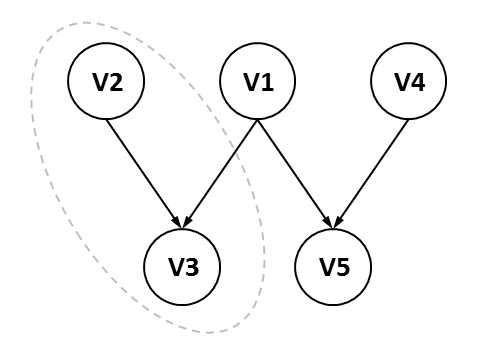
\includegraphics[width=1.6in]{figures/enum_mbpt1.png}
	\caption{MBP duplicated
          during enumeration}
	\label{enum_dup_a}
\end{minipage}
\hfill
\begin{minipage}[b]{0.35\textwidth}
	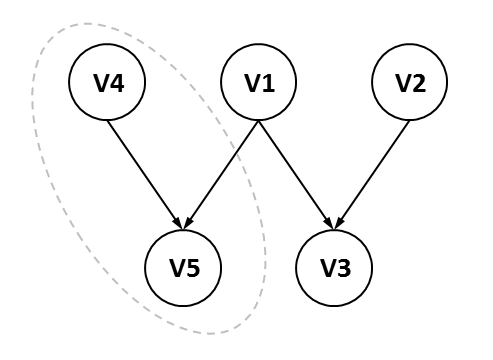
\includegraphics[width=1.6in]{figures/enum_mbpt2.png}
	\caption{Second MBP duplicated
          during enumeration}
	\label{enum_dup_b}
\end{minipage}
\end{figure}

???

As the largest branch is enumerated independently from the remaining
nodes, we double count the case when $k=k'$. For example, we obtain
Figure \ref{enum_dup_a} when labelling the largest branch (i.e.,
left/right) with $\{V2, V3\}$, and Figure \ref{enum_dup_b} when
labelling the largest branch (i.e., left/right) with $\{V4, V5\}$. The
resulting two labeled graphs, however, are identical and hence we
divide the total number by $\frac{1}{2}$. In general, the total
number needs to be divided by $\frac{1}{m}$; hence
$\frac{q}{m}$ appears in equation (\ref{enum_gnmk}).  \qedwhite
\end{proof}

The total number of Markov Blanket polytrees (MBPs) is dramatically reduced comparing with DAGs as shown in Table \ref{tb:nmbps}.

\begin{table}[]
\centering
\caption{The number of labeled DAGs and MBPs on $n \in [0, 7]$ nodes.}
\label{tb:nmbps}
\begin{tabular}{lll}
\hline
\# nodes & \# DAGs    & \# MBPTs \\ \hline
1        & 1          & 1        \\
2        & 3          & 2        \\
3        & 25         & 6        \\
4        & 543        & 23       \\
5        & 29281      & 104      \\
6        & 3781503    & 537      \\
7        & 1138779265 & 3100     \\ \hline
\end{tabular}
\end{table}

The message length for transmitting data using a MBP model is calculated as the natural log of the conditional probability
\begin{align*}
p(X_i|S) = \frac{p(X_i \mid \pi_i^{T_i})\prod_{X_j \in S} p(X_j | \pi_j^{T_i})}{\sum_{x_i=1}^{r_i}p(x_i \mid \pi_i^{T_i})\prod_{X_j \in S} p(X_j | \pi_j^{T_i})}
\end{align*}
is factorized into a product of each variable's probability conditioning on its parents set in a Markov Blanket polytree $T_i$, which can be estimated from data using the adaptive code method. Hence, the total message length has the form 
\begin{align}
\label{eq:mmlmbp}
\begin{split}
I(\phi_i(S), D_{\phi_i}) = -\sum_{D_{\phi_i}} \biggl[
&\ln p(X_i\mid \pi_i^{T_i}) + \sum_{X_j \in S} \ln p(X_j | \pi_j^{T_i}) - \\
&\ln \sum_{x_i=1}^{r_i}p(x_i \mid \pi_i^{T_i})\prod_{X_j \in S} p(X_j | \pi_j^{T_i})
\biggr].
\end{split}
\end{align}
To calculate a weighted average score, we uniformly average the conditional probabilities $p(X_i\mid S)$ over all possible MBPs  $\mathcal{T}_i$ containing the same variables $\{X_i\} \cup MB_i$, then take the negative $\log$ of the expected probability. The uniform prior can be replaced by any reasonable prior over the possible Markov Blanket polytrees.


\subsection{Pseudo-code of the MBMML algorithm}
This section presents the pseudo-code of two types of the MBMML algorithm that learns Markov Blanket of a target variable using either a fixed local structure (i.e., CPT or NB) or an ensemble of random local structures (i.e., MBPs). Both algorithms use a greedy search starting with empty Markov Blanket and iteratively adding the highest ranked candidate into the Markov Blanket to reduce the total message length calculated by a MML metric (equation \ref{eq:mmlcpt} or \ref{eq:mmlnb}, or \ref{eq:mmlmbp}). Both algorithms stop and output a learned Markov Blanket if no scores can be increased by adding more candidates. Algorithms \ref{alg:mbmmlf} and \ref{alg:mbmmlr} outline steps of the fixed and ensemble methods.

\begin{algorithm}[]
\caption{MB discovery using MBMML+CPT/NB}
\label{alg:mbmmlf}
\begin{algorithmic}[MBMML]
\Procedure{$MBMML$}{$X_i, X, D, \phi_i$}, where $X_i$ is the target variable, $X$ is the set of all variables, $D$ is a given dataset and $\phi_i$ is fixed to be either a CPT or  NB model.
    \State $S = X \setminus {X_i}$ \Comment{unchecked variables}
    \State $Z = \emptyset$ \Comment{learned MB}
    \State $L = I(\phi_i(\emptyset), D_{\phi_i})$  \Comment{empty model score}
    \While {$S \neq \emptyset$}
    		\State $X_k = \argmin_{X_j} I(\phi_i(Z \cup \{X_j\}), D_{\phi_i}), \forall X_j \in S$ \Comment{best candidate}
    		\State $L' = I(\phi_i(Z \cup \{X_k\}), D_{\phi_i})$ \Comment{current best score}
    		\If{$L' < L$} \Comment{admit when score reduces}
    			\State $Z = Z \cup \{X_k\}$
    			\State $S = S \setminus \{X_k\}$
    			\State $L = L'$ \Comment{update best score}
    		\Else
    			\State Stop 
			\EndIf
	\EndWhile
	\State Output $Z$
\EndProcedure
\end{algorithmic}
\end{algorithm}

% Insert the algorithm
\begin{algorithm}[]
\caption{MB discovery using MBMML+ENSEMBLE}
\label{alg:mbmmlr}
\begin{algorithmic}[MBMML]
\Procedure{$MBMML$}{$X_i, X, D, \phi_i, K$}, where $X_i$ is the target variable, $X$ is the set of all variables, $D$ is a given dataset, $\phi_i$ is a MBP model, $K$ is the number of randomly sampled MBPs. 
    \State $S = X \setminus {X_i}$ \Comment{unchecked variables}
    \State $Z = \emptyset$ \Comment{learned MB}
    \State $L = I(\phi_i(\emptyset), D_{\phi_i})$  \Comment{empty model score}
    \While {$S \neq \emptyset$}
    		\If{$f(|Z| + 1) \leq K$} \Comment{number of MBPs by equation \ref{eq:nmbps}}
    			\State $\mathcal{T}_i := \{\text{all MBPs over } Z \cup \{X_j\}\}$ \Comment{all MBPs}
    		\Else
    			\State $\mathcal{T}_i =  \{K \text{ random MBPs over } Z \cup \{X_j\}\}$ \Comment{randomly sampled MBPs}
    		\EndIf 
    		\State $X_k = \argmin_{X_j} E_{\mathcal{T}_i}(I(\phi_i(Z \cup \{X_j\}), D_{\phi_i})), \forall X_j \in S$ \Comment{best candidate}
    		\State $L' = E_{\mathcal{T}_i}(I(\phi_i(Z \cup \{X_k\}), D_{\phi_i}))$ \Comment{current best expected score}
    		\If{$L' < L$} \Comment{admit when score reduces}
    			\State $Z = Z \cup \{X_k\}$
    			\State $S = S \setminus \{X_k\}$
    			\State $L = L'$ \Comment{update best score}
    		\Else
    			\State Stop 
			\EndIf
	\EndWhile
	\State Output $Z$
\EndProcedure
\end{algorithmic}
\end{algorithm}

To ensure there is no conflict among the learned Markov Blankets so that they can be used later for structure learning, we enforced outputs from both MBMML+CPT/N and MBMML+ENSEMBLE algorithms to satisfy the symmetry property as shown in section \ref{sec:mb}. There are two deterministic enforcements, by union or intersection between two learned Markov Blankets. The process of the symmetry enforcement is shown in Algorithm \ref{alg:sym}. Throughout these experiments we applied the UNION enforcement to MBMML+CPT, because a CPT model's precision converges to $1$ as sample size increases. So its exponential increase in parameters is likely to result in more false negatives than false positives. The INTERSECTION enforcement was conducted on MBMML+NB, because a Na\"ive Bayes model intend to produce more false positives than a CPT model due to its lack of explanation power, but less false negatives because of its simplicity. It is not clear which enforcement is a better option for MBMML+ENSEMBLE, so we chose the UNION enforcement throughout the experiments. 

\begin{algorithm}[]
\caption{Symmetry enforcement}
\label{alg:sym}
\begin{algorithmic}[]
\Procedure{}{} Given the learned Markov Blankets $\{MB_i\}, \forall X_i \in X$
\For{each $MB_i$}
	\For{each $X_j \in MB_i$}
		\If{$X_i \notin MB_j$}
			\If{UNION}
				\State $MB_j = MB_j \cup \{X_i\}$
			\Else{ INTERSECTION}
				\State $MB_i = MB_i \setminus \{X_j\}$
			\EndIf
		\EndIf
	\EndFor
\EndFor
	\State Output $\{MB_i\}$
\EndProcedure
\end{algorithmic}
\end{algorithm}


\section{Experiments on Markov Blanket discovery}
In this section, we present some of the experimental results on comparing different Markov Blanket learners. All three algorithms, MBMML+CPT, MBMML+NB, and MBMML+ENSEMBLE were tested against the following algorithms: 
\begin{itemize}
\item IAMB - a constraint-based algorithm that uses conditional independence test for candidate admission. It starts admitting variables that are dependent with the target conditioning on the current found Markov Blanket. It is followed by a backward phase trying to delete any false positives.  
\item PCMB - a constraint-based algorithm that divides a learning into two sub-tasks. Firstly, it finds the direct neighbors of the target. It then finds the neighbors of each neighbor of the target, and prunes any false positives. This algorithm also relies on conditional independence test. 
\item SLL - a metric-based algorithm that uses dynamic programming and BDeu score. It is an exact algorithm that searches through the entire space of equivalence classes of local DAGs around a target, then reads off the optimal Markov Blanket. Notice SLL does not just learn Markov Blankets. It is for scaling up Bayesian network structure learning. 
\end{itemize}
We used the implementations of IAMB and PCMB provided by \cite{pena2007towards} and setted the significant level $\alpha=0.05$ for conditional independence test. We used SLL's source code provided by \cite{niinimaki2012local} and its default equivalent sample size $1$ for BDeu. SLL fallbacks to GES algorithm \cite{chickering2002learning} if it tends to find more than $20$ variables for a Markov Blanket. The three MML methods assumed uniform parameter prior (i.e., symmetric Dirichlet with concentration parameter $\vec{\alpha} = <1>$). The MBMML+ENSEMBLE algorithm was setted to randomly sample $100$ Markov Blanket polytrees from the entire space and uniformly averaged their message lengths. 
%The IPCMB algorithm has been experimentally justified to outperform IAMB and PCMB. And the IPCMB recently has been justified to be less superior than SLL and STMB \cite{gao2017efficient} on similar datasets. 

Section \ref{sec:exp_real} focuses on testing with real models (Table \ref{tab:exp_models})and standard datasets provided by \footnote{\url{http://www.dsl-lab.org/supplements/mmhc_paper/mmhc_index.html\#complete_data}}. The sample size varies in $500, 1000, 5000$ and each size comes with $10$ different datasets. These models are often used for testing Markov Blanket and causal discovery learners.  Section \ref{sec:exp_artificial} extends the experiments to artificial Bayesian networks (\ref{tab:exp_models}) containing $30$ and $50$ variables respectively, and the same maximum fan-in and number of states for each variable. For each model specification, we randomly generate $5$ different Bayesian networks, each of which was then used to generate $5$ different datasets for every one of the sample sizes $100, 500, 2000, 5000$. 

The evaluation metrics used are precision, recall, and edit distance. The edit distance between a true Markov Blanket and a learned Markov Blanket is equal to the sum of false positives and false negatives. The average accuracy over all variables in one structure and all samples with the same size were reported with $95\%$ confidence intervals. Due to space limit, only selected models were discussed in the main text. The rest of the results are included in the appendix. 
\begin{table}
% table caption is above the table
\caption{Summary of tested Bayesian networks. 30-5-4-1 and 30-5-4-1 refer to artificial networks with 30 and 50 variables, maximum fan-in 5, maximum number of states 4, and uniform ($\vec{\alpha}=<1>$) parameter prior.}
\label{tab:exp_models}       
\begin{tabular}{llll}
\hline\noalign{\smallskip}
Network    & Number of odes & Max fan-in & Mean MB size  \\
\noalign{\smallskip}\hline\noalign{\smallskip}
CHILD      & 20    & 2  &  3 \\
INSURANCE & 27    & 3  &  5.19 \\
ALARM     & 37   & 4  & 3.51 \\  
BARLEY & 48 & 4 & 5.25 \\
HAILFINDER & 56 & 4 & 3.54 \\
30-5-4-1 & 30 & 5 & 8 \\
50-5-4-1 & 50 & 5 & 9.73 \\
\noalign{\smallskip}\hline
\end{tabular}
\end{table}


\subsection{Accuracy on real models}
\label{sec:exp_real}
Figures \ref{fg:child} and \ref{fg:barley} report the mean edit distance (with confidence intervals) of all algorithms on the CHILD and BARLEY networks. In both cases, IAMB has the lowest accuracy given any sample size. In most cases, the other algorithms show no statistically significant difference from each other, except PCMB and MML+ENSEMBLE are less robust under small samples. Both PCMB and SLL have shown a projection of faster convergence than MML methods and IAMB. Noticing that PCMB failed to run on the BARLEY network possibly due to an implementation error. The edit distance and precision and reacall on all five models are summarized in Table \ref{tb:all_ed} and Table \ref{tb:all_pre_rec} (in appendix) respectively. In general, on these real networks SLL has most of the winnings followed, MBMML+CPT, MBMML+NB, PCMB, MBMML+ENSEMBLE and IAMB. 
\begin{figure}[htb]
  \centering
    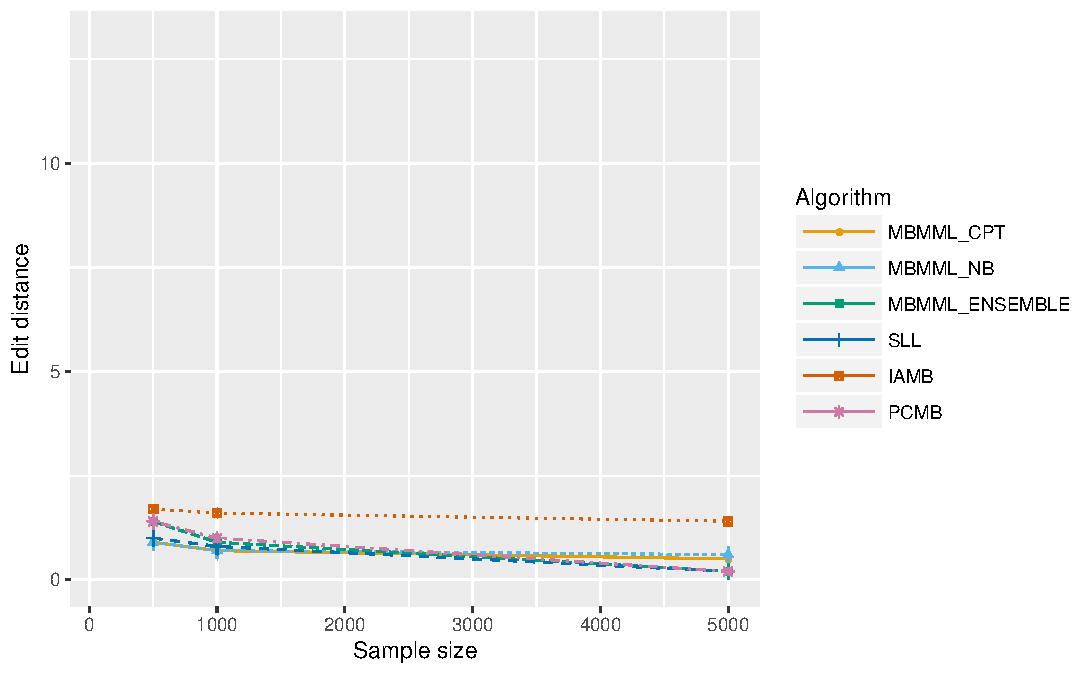
\includegraphics[scale=0.6]{figures/ed_vs_samplesize_child.pdf}
  \caption{Edit distance (with $95\%$ confidence intervals) v.s. sample size on CHILD network.}
  \label{fg:child}
\end{figure}

\begin{figure}[hbt]
  \centering
    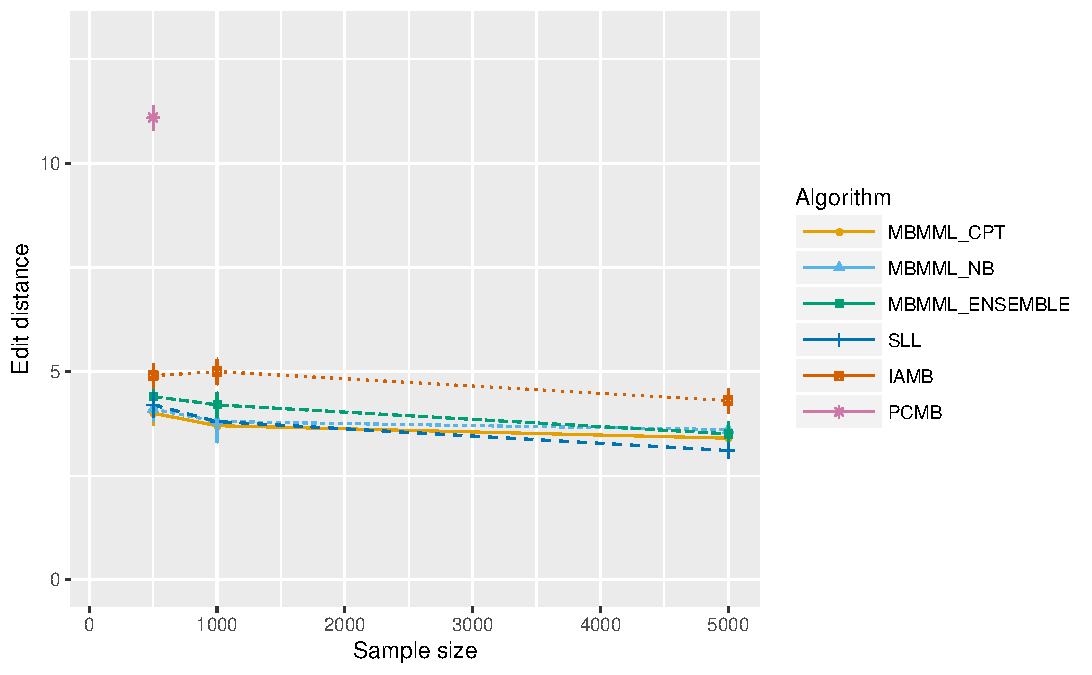
\includegraphics[scale=0.6]{figures/ed_vs_samplesize_barley.pdf}
  \caption{Edit distance (with $95\%$ confidence intervals) v.s. sample size on BARLEY network. PCMB failed under 1000 and 5000 samples possibly due to an implementation error.}
  \label{fg:barley}
\end{figure}

\subsection{Accuracy on artificial models} 
\label{sec:exp_artificial}
To test all metods on different problems over a number of random networks, we generated 5 different Bayesian networks for each pre-specified model specification. These networks are moderate in the number of nodes, and slightly larger comparing with the real networks used before in maximum fan-in and average Markov Blanket size. Their parameters were sampled from uniform distribution which matches the parameter prior used in the multi-state MML metric. This may be an advantage of the MML methods for these particular problems, but it is less risky when nothing is known about the models. Later in this section, it has been shown briefly that this uninformative prior could produce similar accuracy as using the true prior.  

Figure \ref{fg:30} and \ref{fg:50} have shown how the tested methods reacted to different sample sizes on artificial networks with specification 30-5-4-1 and 50-5-4-1. The MBMML+NB and IAMB algorithms started well under extreme small samples but could not converge given more samples. This is likely to be caused by the lack of representation power of Naive Bayes models and the unsoundness of IAMB. The MBMML+CPT and MBMML+ENSEMBLE algorithms have shown competitive performances under both small and large samples, and superior low edit distance for moderate samples, but both methods converged slower than PCMB and SLL towards 5000 samples. The main issue is believed to be the exponential number of parameters in both CPT and MBPT models. Both PCMB and SLL converged faster than the others like in the real model cases. The former, however, had the worst accuracy under 100 samples whilst the later are  almost no difference from the others. 
\begin{figure}[hbt]
  \centering
    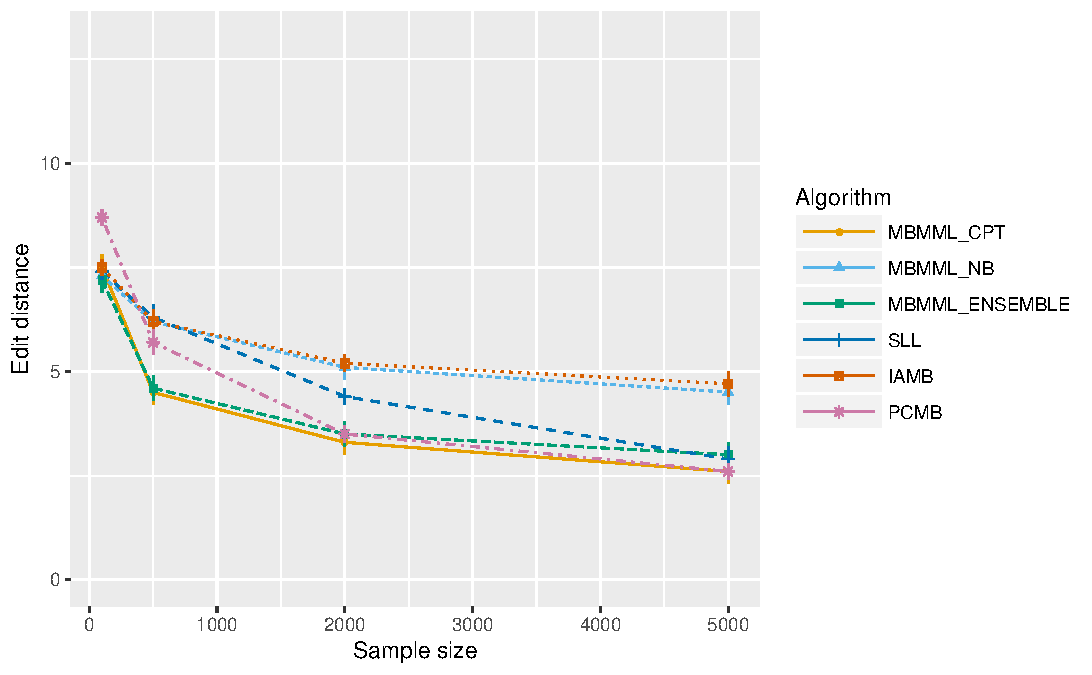
\includegraphics[scale=0.6]{figures/ed_vs_samplesize_30_5_4_1.pdf}
  \caption{Edit distance (with $95\%$ confidence intervals) v.s. sample size on artificial Bayesian networks (30-5-4-1) containing 30 variables, maximum 5 parents and maximum 4 states for each variable.}
  \label{fg:30}
\end{figure}

\begin{figure}[hbt]
  \centering
    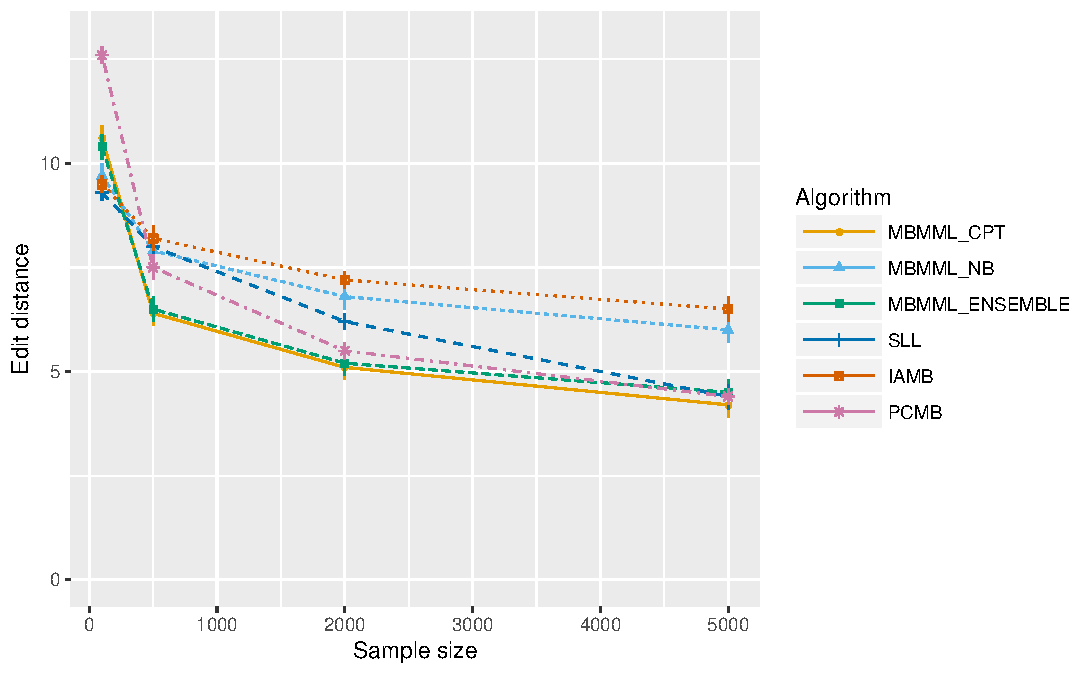
\includegraphics[scale=0.6]{figures/ed_vs_samplesize_50_5_4_1.pdf}
  \caption{Edit distance (with $95\%$ confidence intervals) v.s. sample size on artificial Bayesian networks (50-5-4-1) containing 50 variables, maximum 5 parents and maximum 4 states for each variable.}
  \label{fg:50}
\end{figure}

So far, we have investigated the overall performance of Markov Blanket learners given some networks. Now, we group together problems having similar complexity and look for the trend when increasing Markov Blanket size. Figure \ref{fg:ed_mb_50_500} and \ref{fg:ed_mb_50_5000} are edit distances of all methods for different Markov Blanket size given 500 and 5000 samples respectively. The rest of the results are contained in the appendix.  

\begin{figure}[hbt]
  \centering
    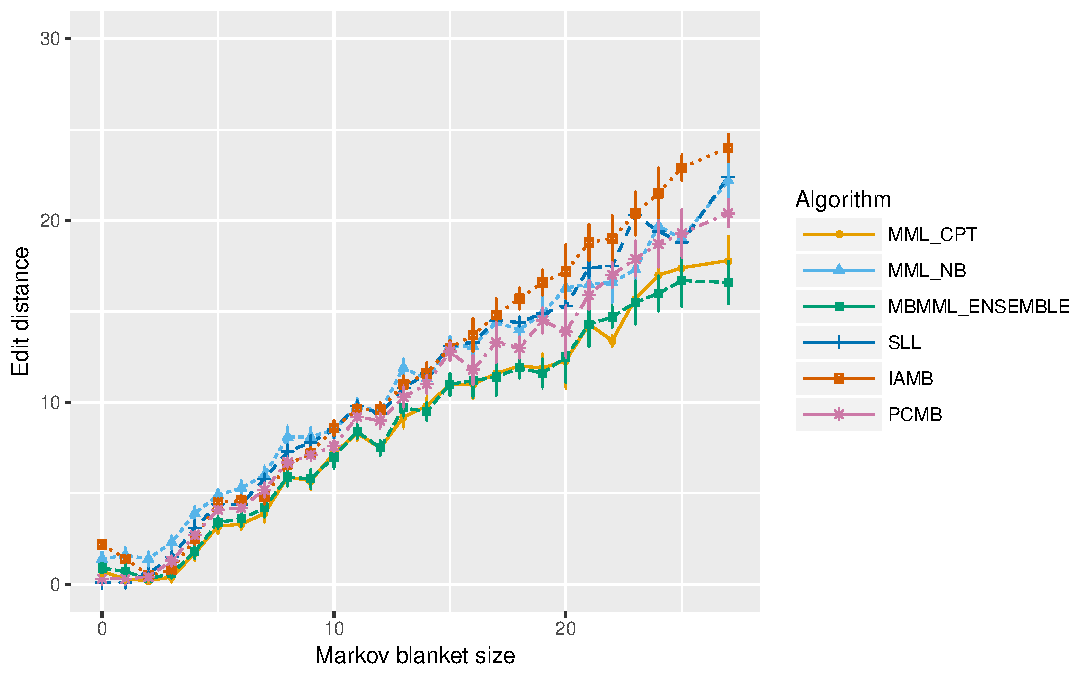
\includegraphics[scale=0.6]{figures/ed_vs_mbsize_50_5_4_1_500.pdf}
  \caption{Edit distance against Markov Blanket size on 50-5-4-1 models with 500 samples.}
  \label{fg:ed_mb_50_500}
\end{figure} 
Given 500 samples (Figure \ref{fg:ed_mb_50_500}) for 50 variables networks, PCMB and SLL did well by identifying unconnected variables, whilst the others more or less had some false positives. As Markov Blanket size was increased, the MBMML+CPT and MBMML+ENSEMBLE algorithms produced the fewest false findings all the way up to the maximum Markov Blankets. It is worth noticing that for Markov Blankets over 20 variables, it is GES's performance instead of SLL. On averaged, MBMML+CPT and MBMML+ENSEMBLE have the lowest edit distance which is consistent with the ranking in Figure \ref{fg:50} for 500 samples. 

\begin{figure}[hbt]
  \centering
    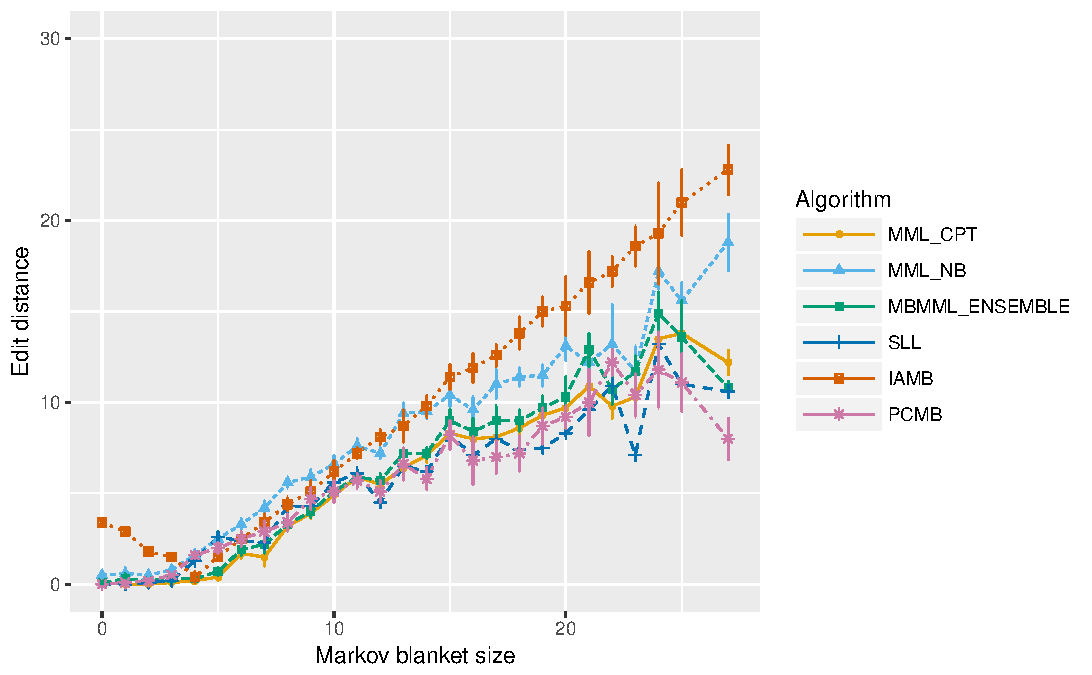
\includegraphics[scale=0.6]{figures/ed_vs_mbsize_50_5_4_1_5000.pdf}
  \caption{Edit distance against Markov Blanket size on 50-5-4-1 models with 5000 samples.}
  \label{fg:ed_mb_50_5000}
\end{figure}
Given 5000 samples (Figure \ref{fg:ed_mb_50_5000}), most methods did well for Markov Blanket size smaller than 4 except IAMB, who had a wired U-shape where the bottom is at 4 variables. MBMML+CPT and MBMML+ENSEMBLE kept the lowest edit distance for medium Markov Blankets, but were unable to keep it low as the learning problems became more complex so being outperformed occasionally by PCMB and SLL. In summary, the two MML methods except MBMML+NB have lowest error rate for medium-sized learning problems given moderate samples. 

There may be a concern that if the generating models used a non-uniform prior, the MML methods could produce different results. In principle, if the true prior is not uniform, using uniform prior would give no better results than uing the true prior. In practice, however, it is also depends on the quality and size of samples. To show the impact of using uninformative prior, MBMML+CPT was given both the true prior and uniform prior then tested on a 30-5-4-1 network whose parameters were sampled from a symmetric Dirichlet distribution with different concentration parameter $\alpha \in \{0.1, 0.4, 0.7, 1, 10, 40, 70, 100\}$. The experiments were completed for 500 and 5000 samples. 

Figure \ref{fg:wrong_prior_500} and \ref{fg:wrong_prior_5000} have shown insiginificant difference between the use of true prior and uniform prior for the case when the concentration parameters $\alpha \le 1$. This is because adding small $\alpha$ values to parameter estimations almost do not matter when there exists at last some data for each parameter. When $\alpha > 1$, uniform prior produced slightly less edit distance than the true prior. By looking into the number of learned Markov Blanket size, we notice that as $\alpha$ increases the learned Markov Blankets also increase in size. It is believed that this is caused by the same reason as the sensitivity of BDeu as shown by \cite{silander2007sensitivity}. The MML metric for CPT model with symmetric Dirichlet prior is similar as the BDeu metric, except the former includes costs for stating estimated parameters and used uniform Dirichlet prior over all model parameters whilst the later does not state parameters and only used uniform Dirichlet prior over parameters of each node. But both metrics penalise model complexity using a function of $\alpha$, which decreases as $\alpha$ increases. Hence, under large $\alpha$ the MML methods discovered larger Markov Blankets which could contain a large propotion of false positives especially under small samples. This is also why when using 5000 samples, the true prior produced similar edit distance as uniform prior.

\begin{figure}[hbt]
  \centering
    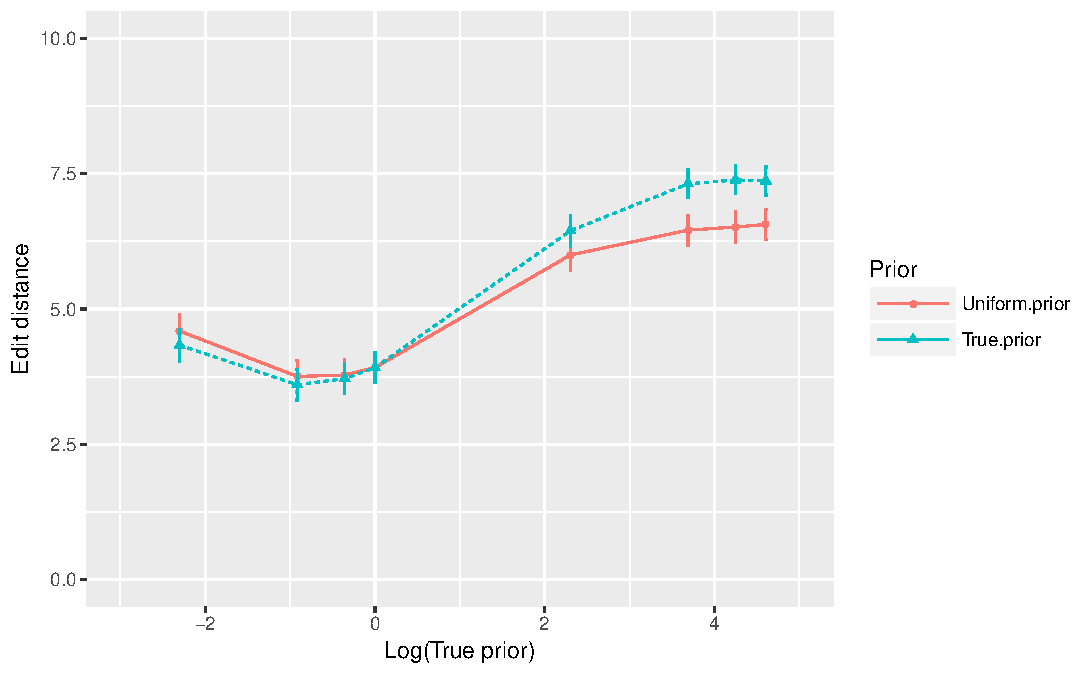
\includegraphics[scale=0.6]{figures/ed_vs_trueprior_30_5_4_alpha_134445_500.pdf}
  \caption{MBMML+CPT's edit distances using the true prior and uniform prior on a 30-5-4-1 model with 500 samples. The X-axis is the natural log scale of the true symmetric Dirichlet concentration parameter $\alpha = \{0.1, 0.4, 0.7, 1, 10, 40, 70, 100\}$.}
  \label{fg:wrong_prior_500}
\end{figure}

\begin{figure}[hbt]
  \centering
    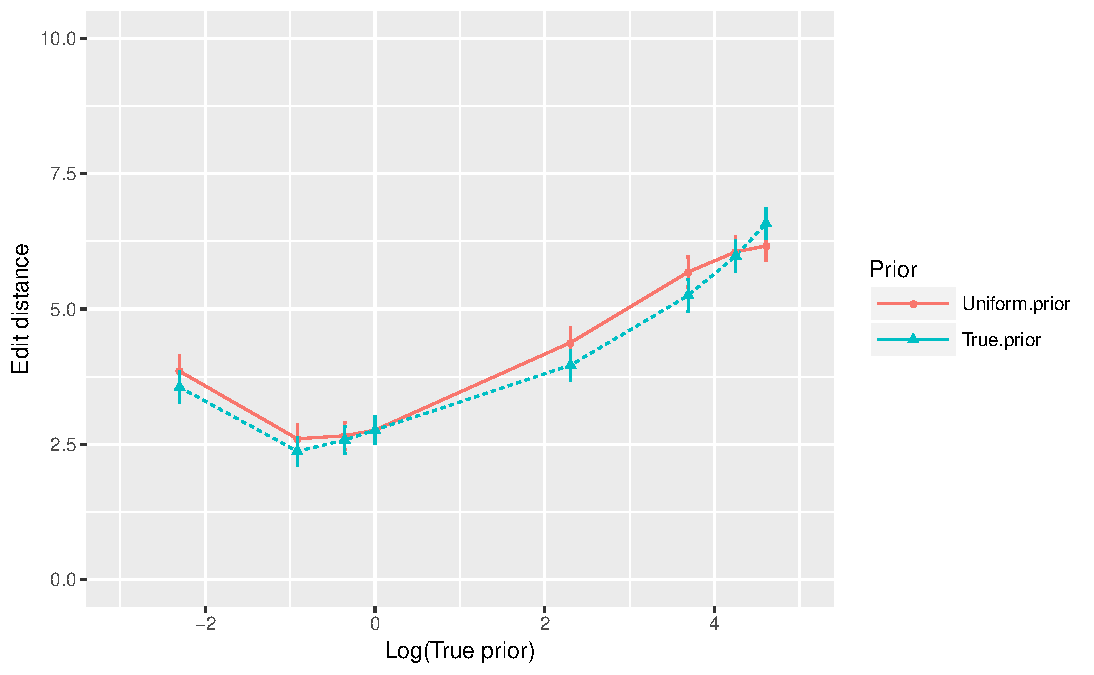
\includegraphics[scale=0.6]{figures/ed_vs_trueprior_30_5_4_alpha_134445_5000.pdf}
  \caption{MBMML+CPT's edit distances using the true prior and uniform prior on a 30-5-4-1 model with 5000 samples. The X-axis is the natural log scale of the true symmetric Dirichlet concentration parameter $\alpha = \{0.1, 0.4, 0.7, 1, 10, 40, 70, 100\}$.}
  \label{fg:wrong_prior_5000}
\end{figure}

\subsection{Algorithm complexity}
Table \ref{tb:bigo} orders all algorithms by ascending computational complexity. The while loop in Algorithm \ref{alg:mbmmlf} runs at most $n-1$ times. Each time it runs through all unchecked nodes to find the best candidate according to a MML metric. For a CPT model, there could be at most $n-1$ parents in which case the multi-state MML is summed over all $2^{n-1}$ parents instantiations. So the computational complexity of the MBMML+CPT algorithm is $O(n2^{n-1})$. For a NB model, the worst case is when all $n-1$ nodes are children of the target, which is linear in $n$ within the \textit{WHILE} loop, so gives a complexity $O(n^2)$. The worst case of MBMML+RANDOM is when a CPT model appears in the sampled Markov Blanket polytrees. In general, a random model is slower than a CPT by a constant factor, which is determined by the number of sampled local structures. But it has the same complexity as a CPT model. For PCMB, the total time required is dominated by the process of finding the direct neighbors of the target. This process tries to find a subset of the neighbor set, conditioning on which the target is independent with a candidate. And such a process runs through all variables to ensure the symmetry property. Hence, its complexity in the worst case is $O(n^2 2^{n-1})$. The total time required by IAMB and SLL were published in the associated papers. 
\begin{table}[]
\centering
\caption{Algorithm's computational complexity in big O notation.}
\label{tb:bigo}
\begin{tabular}{ll}
\hline
Algorithm    & Big O notation \\ \hline
IAMB      & $O(n^2)$      \\
MBMML+NB          &    $O(n^2)$    \\
MBMML+CPT          &   $O(n2^{n-1})$      \\
MBMML+RANDOM         & $O(n2^{n-1})$        \\
PCMB & $O(n^2 2^{n-1})$     \\
SLL        & $O(n^4 2^n)$       \\ \hline 
\end{tabular}
\end{table}


\section{Conclusion}
\label{sec:disc}

This paper presented three MML methods for learning Markov Blankets of
variables. The three methods are all built based on the multi-state
MML metric, but associated with different models that are CPT, Naive
Bayes and an ensemble of random Markov Blanket polytree models. The
MBMML+CPT algorithm was proven to be correct under infinite samples,
though may not be data efficient for large Markov Blankets due to
exponential number of parameters. The MBMML+NB algorithm was developed
to overcome the problem of exponential model complexity by sacrificing
the the modelling of variable interactions. Both methods have no
tendency of learning the subgraphs within Markov Blankets, although
certain model structures are assumed during learning. Realizing it is
restricted to consider only a particular model structure for learning
Markov Blankets, we generalized to the MBMML+ENSEMBLE algorithm that
assesses the validity of a variable being in a Markov Blanket under
random polytrees within Markov Blankets. The search algorithms used
are greedy search but can be replaced with any heuristics or
probabilistic searches. The three MML algorithms were tested against
several other Markov Blanket algorithms on both real and artificial
Bayesian networks given different sample sizes. In general, MBMML+CPT
and MBMML+ENSEMBLE show superior results given moderate samples than
the others. In particular, they had the lowest edit distance when
learning medium-sized Markov Blankets. The method with Naive Bayes
model occationally appeared to be competitive for very small samples
but could not converge given more samples. Comparing with the
approximate algorithm PCMB, the two MML methods have advantages in
both accuracy and efficiency, especially under small and medium
samples. Comparing with the exact learning algorithm SLL, they are
competitive in accuracy and faster in computational complexity by a
factor of $n^3$.

%In this paper, we proposed the \mbptmml algorithm that uses local-to-global paradigm to scale up general causal discovery algorithm to larger models with encouraging accuracy. \mbptmml's local step focuses on learning a local structure named MBPTs, the total number of which has been proved to be sub-exponential comparing with DAGs. Empirical evaluations against local-to-global and general causal learners suggested that \mbptmml is a competitive algorithm in most cases with some exceptions perhaps because of inappropriate prior used in MML. Although the test on execution time is not rigorous enough, meaning there are other factors such as machine specification, proper analysis of speed different between programming languages etc., that could have been controlled. It provides an estimation of \mbptmml's efficiency comparing with other types of learns, especially when comparing with those that adopted dynamic programming for optimal output. Although the current results are promising, \mbptmml has rooms to be improved. We have shown that inaccurate local variable and structure learnings can easily deviate a LGL learner from converging to generating models. To overcome this problem, we will consider several different roles of a new node in a MBPT structure to obtain an averaged prediction to a target. We believe this could avoid having a full CPT and hence further improve the recall of the current \mmlcpt process. The current version of \mbptmml extends onto global structures in a deterministic way, a potential improvement is to consider this step probabilistically such as giving these local adjacencies to CaMML as prior, hence reduce CaMML's sampling space so that models with higher posterior probability will be more accurately estimated in CaMML's MCMC step. By doing so, CaMML will be enabled to learn larger models that the current CaMML failed to do such as in CHILD5 and ALARM5. 


\newpage
\section{appendix}

\begin{table}[]
\centering
\caption{Summary of edit distance (with $95\%$ confidence intervals) of all Markov Blanket discovery algorithms on both real and artificial Bayesian networks. The best results are highlighted in grey. In real networks, SLL wins most of the times followed by MBMML+CPT, MBMML+NB, PCMB, MMLL+ENSEMBLE, IAMB. PCMB failed to learn on BARLEY networks under 1000 and 5000 samples possibly due to an implementation error. In artificial networks, MBMML+CPT and MBMML+ENSEMBLE win most of the times followed by SLL, PCMB, MBMML+NB, IAMB.}
\label{tb:all_ed}
\begin{tabular}{llllllll}
\hline
Network    & SAMPLES &  \begin{tabular}[c]{@{}l@{}}$MBMML$\\ $+CPT$\end{tabular} &  \begin{tabular}[c]{@{}l@{}}$MBMML$\\ $+NB$\end{tabular} & \begin{tabular}[c]{@{}l@{}}$MBMML$\\ $+ENSEMBLE$\end{tabular} & IAMB     & PCMB     & SLL      \\ \hline
CHILD      & 500     & \cellcolor{lightgray}0.9+-0.2      & \cellcolor{lightgray}0.9+-0.2     & 1.4+-0.2  & 1.7+-0.2 & 1.4+-0.2 & \cellcolor{lightgray}1+-0.2   \\
           & 1000    & \cellcolor{lightgray}0.7+-0.1      & \cellcolor{lightgray}0.7+-0.2     & \cellcolor{lightgray}0.9+-0.2  & 1.6+-0.2 & \cellcolor{lightgray}1+-0.2   & \cellcolor{lightgray}0.8+-0.1 \\
           & 5000    & 0.5+-0.1      & 0.6+-0.1     & \cellcolor{lightgray}0.2+-0.1  & 1.4+-0.2 & \cellcolor{lightgray}0.2+-0.1 & \cellcolor{lightgray}0.2+-0.1 \\ \hline
INSURANCE  & 500     & \cellcolor{lightgray}3.3+-0.2      & \cellcolor{lightgray}3.5+-0.2     & 3.7+-0.3  & \cellcolor{lightgray}3.6+-0.3 & \cellcolor{lightgray}3.4+-0.2 & \cellcolor{lightgray}3.1+-0.2 \\
           & 1000    & \cellcolor{lightgray}2.9+-0.2      & 3.3+-0.2     & \cellcolor{lightgray}3.1+-0.3  & 3.7+-0.3 & \cellcolor{lightgray}3+-0.2   & \cellcolor{lightgray}2.7+-0.2 \\
           & 5000    & \cellcolor{lightgray}2.1+-0.2      & 2.8+-0.2     & 2.4+-0.2  & 2.8+-0.2 & \cellcolor{lightgray}1.8+-0.2 & \cellcolor{lightgray}2+-0.2   \\ \hline
ALARM      & 500     & 1.4+-0.1      & 2.1+-0.2     & 2.3+-0.2  & 2.2+-0.2 & 1.7+-0.2 & \cellcolor{lightgray}0.8+-0.1 \\
           & 1000    & 1+-0.1        & 1.8+-0.2     & 1.9+-0.2  & 2+-0.2   & 1.1+-0.1 & \cellcolor{lightgray}0.6+-0.1 \\
           & 5000    & 0.5+-0.1      & 1.5+-0.2     & 1.5+-0.1  & 1.5+-0.2 & \cellcolor{lightgray}0.2+-0.1 & \cellcolor{lightgray}0.2+-0   \\ \hline
BARLEY     & 500     & \cellcolor{lightgray}4+-0.3        & \cellcolor{lightgray}4.1+-0.3     & \cellcolor{lightgray}4.4+-0.3  & 4.9+-0.3 & 11.1+-0.5 & \cellcolor{lightgray}4.2+-0.2 \\
           & 1000    & \cellcolor{lightgray}3.7+-0.3      & \cellcolor{lightgray}3.8+-0.3     & \cellcolor{lightgray}4.2+-0.3  & 5+-0.3 & NA & \cellcolor{lightgray}3.8+-0.2 \\
           & 5000    & \cellcolor{lightgray}3.4+-0.3      & \cellcolor{lightgray}3.6+-0.3     & \cellcolor{lightgray}3.5+-0.3  & 4.3+-0.3 & NA & \cellcolor{lightgray}3.1+-0.2 \\ \hline
HAILFINDER & 500     & \cellcolor{lightgray}4.4+-0.3      & \cellcolor{lightgray}4.3+-0.2      & 5.2+-0.3  & \cellcolor{lightgray}4.2+-0.2 & 7.6+-0.5 & \cellcolor{lightgray}4.3+-0.3 \\
           & 1000    & \cellcolor{lightgray}4.4+-0.3      & \cellcolor{lightgray}4.3+-0.2     & 5+-0.3    & \cellcolor{lightgray}4.5+-0.2 & 6.7+-0.4 & \cellcolor{lightgray}4.1+-0.3 \\
           & 5000    & \cellcolor{lightgray}4.3+-0.3      & \cellcolor{lightgray}4.3+-0.2       & 5.1+-0.3  & 5.1+-0.2 & \cellcolor{lightgray}3.9+-0.2 & \cellcolor{lightgray}4+-0.3  \\ \hline
30-5-4-1   & 100     & \cellcolor{lightgray}7.5+-0.3      & \cellcolor{lightgray}7.3+-0.3     & \cellcolor{lightgray}7.2+-0.3  & \cellcolor{lightgray}7.5+-0.3 & 8.7+-0.3 & \cellcolor{lightgray}7.4+-0.3 \\
		   & 500     & \cellcolor{lightgray}4.5+-0.3      & 6.3+-0.3     & \cellcolor{lightgray}4.6+-0.3  & 6.2+-0.3 & 5.7+-0.3 & 6.3+-0.3 \\
           & 2000    & \cellcolor{lightgray}3.3+-0.2      & 5.1+-0.3     & \cellcolor{lightgray}3.5+-0.2  & 5.2+-0.3 & \cellcolor{lightgray}3.5+-0.2 & 4.4+-0.3 \\
           & 5000    & \cellcolor{lightgray}2.6+-0.2      & 4.5+-0.2     & \cellcolor{lightgray}3+-0.2    & 4.7+-0.3 & \cellcolor{lightgray}2.6+-0.2 & \cellcolor{lightgray}2.9+-0.2 \\ \hline
50-5-4-1   & 100     & 10.66+-0.3      & \cellcolor{lightgray}9.7+-0.3     & 10.4+-0.3  & \cellcolor{lightgray}9.5+-0.3 & 12.6+-0.3 & \cellcolor{lightgray}9.3+-0.3   \\
		   & 500     & \cellcolor{lightgray}4.5+-0.3      & 6.3+-0.3     & \cellcolor{lightgray}4.6+-0.3  & 6.2+-0.3 & 5.7+-0.3 & 6.3+-0.3 \\
           & 2000    & \cellcolor{lightgray}5.1+-0.2      & 6.9+-0.3     & \cellcolor{lightgray}5.2+-0.2  & 7.2+-0.3 & \cellcolor{lightgray}5.5+-0.2 & 6.2+-0.3 \\
           & 5000    & \cellcolor{lightgray}4.2+-0.2      & 6.1+-0.2     & \cellcolor{lightgray}4.5+-0.2  & 6.5+-0.3 & \cellcolor{lightgray}4.4+-0.2 & \cellcolor{lightgray}4.4+-0.2 \\ \hline
\end{tabular}
\end{table}

\begin{landscape}
%\begin{table}[]
\begin{center}
\scalebox{0.7}{
\label{tb:all_pre_rec}
\begin{tabular}{llllllllllllll}
\hline
Network    & SAMPLES & \multicolumn{2}{c}{MBMML+CPT}                          & \multicolumn{2}{c}{MBMML+NB}                           & \multicolumn{2}{c}{MBMML+RANDOM}                              & \multicolumn{2}{c}{IAMB}                                   & \multicolumn{2}{c}{PCMB}                                   & \multicolumn{2}{c}{SLL}                                    \\
           &         & \multicolumn{1}{c}{Precision} & \multicolumn{1}{c}{Recall} & \multicolumn{1}{c}{Precision} & \multicolumn{1}{c}{Recall} & \multicolumn{1}{c}{Precision} & \multicolumn{1}{c}{Recall} & \multicolumn{1}{c}{Precision} & \multicolumn{1}{c}{Recall} & \multicolumn{1}{c}{Precision} & \multicolumn{1}{c}{Recall} & \multicolumn{1}{c}{Precision} & \multicolumn{1}{c}{Recall} \\ \hline
CHILD      & 500     & 0.94+-0.03                    & 0.8+-0.04                  & 0.94+-0.03                    & 0.82+-0.04                 & 0.76+-0.04                    & 0.89+-0.03                 & 0.83+-0.04                    & 0.73+-0.04                 & 0.83+-0.04                    & 0.81+-0.04                 & 0.94+-0.03                    & 0.78+-0.04                 \\
           & 1000    & 0.98+-0.02                    & 0.88+-0.03                 & 0.97+-0.02                    & 0.86+-0.03                 & 0.82+-0.03                    & 0.96+-0.01                 & 0.81+-0.03                    & 0.81+-0.03                 & 0.91+-0.03                    & 0.84+-0.03                 & 0.97+-0.02                    & 0.84+-0.03                 \\
           & 5000    & 1+-0.01                       & 0.91+-0.02                 & 1+-0.01                       & 0.89+-0.02                 & 0.95+-0.02                    & 1+-0                       & 0.77+-0.04                    & 0.91+-0.02                 & 0.98+-0.01                    & 0.99+-0.01                 & 1+-0                          & 0.97+-0.01                 \\ \hline
INSURANCE  & 500     & 0.82+-0.04                    & 0.48+-0.03                 & 0.8+-0.04                     & 0.42+-0.03                 & 0.7+-0.04                     & 0.6+-0.03                  & 0.86+-0.03                    & 0.44+-0.03                 & 0.75+-0.04                    & 0.52+-0.03                 & 0.83+-0.04                    & 0.51+-0.04                 \\
           & 1000    & 0.86+-0.03                    & 0.54+-0.03                 & 0.85+-0.04                    & 0.45+-0.03                 & 0.76+-0.03                    & 0.65+-0.03                 & 0.78+-0.03                    & 0.5+-0.03                  & 0.79+-0.04                    & 0.56+-0.03                 & 0.88+-0.03                    & 0.58+-0.03                 \\
           & 5000    & 0.95+-0.01                    & 0.68+-0.03                 & 0.93+-0.02                    & 0.57+-0.03                 & 0.82+-0.03                    & 0.76+-0.03                 & 0.86+-0.02                    & 0.66+-0.03                 & 0.93+-0.03                    & 0.71+-0.03                 & 0.98+-0.01                    & 0.69+-0.03                 \\ \hline
ALARM      & 500     & 0.85+-0.03                    & 0.77+-0.03                 & 0.79+-0.03                    & 0.67+-0.03                 & 0.66+-0.03                    & 0.87+-0.02                 & 0.81+-0.03                    & 0.65+-0.03                 & 0.84+-0.03                    & 0.71+-0.03                 & 0.92+-0.02                    & 0.89+-0.02                 \\
           & 1000    & 0.9+-0.02                     & 0.82+-0.03                 & 0.86+-0.02                    & 0.68+-0.03                 & 0.69+-0.03                    & 0.92+-0.02                 & 0.81+-0.02                    & 0.75+-0.03                 & 0.9+-0.02                     & 0.81+-0.03                 & 0.94+-0.01                    & 0.94+-0.01                 \\
           & 5000    & 0.97+-0.01                    & 0.93+-0.02                 & 0.95+-0.02                    & 0.7+-0.03                  & 0.75+-0.02                    & 0.95+-0.01                 & 0.79+-0.02                    & 0.89+-0.02                 & 1+-0                          & 0.96+-0.01                 & 0.98+-0.01                    & 0.98+-0.01                 \\ \hline
BARLEY     & 500     & 0.74+-0.03                    & 0.37+-0.03                 & 0.74+-0.03                    & 0.35+-0.02                 & 0.66+-0.03                    & 0.51+-0.03                 & 0.7+-0.04                            & 0.17+-0.01                         & 0.25+-0.01                            & 0.59+-0.03                         & 0.63+-0.04                    & 0.25+-0.02                 \\
           & 1000    & 0.79+-0.03                    & 0.42+-0.03                 & 0.79+-0.03                    & 0.37+-0.02                 & 0.68+-0.03                    & 0.57+-0.03                 & 0.63+-0.04                            & 0.19+-0.02                         & NA                            & NA                         & 0.72+-0.04                    & 0.35+-0.03                 \\
           & 5000    & 0.8+-0.03                     & 0.52+-0.03                 & 0.81+-0.03                    & 0.47+-0.02                 & 0.72+-0.03                    & 0.7+-0.03                  & 0.73+-0.03                            & 0.36+-0.03                         & NA                            & NA                         & 0.85+-0.03                    & 0.5+-0.03                  \\ \hline
HAILFINDER & 500     & 0.3+-0.03                     & 0.18+-0.02                 & 0.25+-0.03                    & 0.12+-0.01                 & 0.27+-0.03                    & 0.2+-0.02                  & 0.31+-0.03                            & 0.17+-0.02                         & 0.28+-0.03                            & 0.19+-0.02                         & 0.28+-0.03                    & 0.14+-0.02                 \\
           & 1000    & 0.31+-0.03                    & 0.22+-0.02                 & 0.26+-0.03                    & 0.12+-0.01                 & 0.29+-0.03                    & 0.24+-0.02                 & 0.29+-0.03                            & 0.19+-0.02                         & 0.32+-0.03                            & 0.21+-0.02                         & 0.3+-0.03                     & 0.18+-0.02                 \\
           & 5000    & 0.34+-0.03                    & 0.26+-0.02                 & 0.26+-0.03                    & 0.14+-0.02                 & 0.3+-0.03                     & 0.27+-0.03                 & 0.24+-0.02                            & 0.23+-0.02                         & 0.32+-0.03                            & 0.21+-0.02                         & 0.34+-0.03                    & 0.22+-0.02                 \\ \hline
30-5-4-1   & 100     & 0.56+-0.02                    & 0.36+-0.02                 & 0.6+-0.03                     & 0.23+-0.02                 & 0.58+-0.02                    & 0.36+-0.02                 & 0.69+-0.03                    & 0.16+-0.01                 & 0.43+-0.02                    & 0.37+-0.02                 & 0.5+-0.03                     & 0.17+-0.02                 \\
           & 500     & 0.91+-0.02                    & 0.56+-0.02                 & 0.86+-0.02                    & 0.35+-0.02                 & 0.86+-0.02                    & 0.56+-0.02                 & 0.84+-0.02                    & 0.37+-0.02                 & 0.87+-0.02                    & 0.41+-0.02                 & 0.79+-0.03                    & 0.3+-0.02                  \\
           & 2000    & 0.97+-0.01                    & 0.68+-0.02                 & 0.94+-0.01                    & 0.48+-0.02                 & 0.94+-0.01                    & 0.68+-0.02                 & 0.89+-0.02                    & 0.51+-0.02                 & 0.93+-0.01                    & 0.69+-0.02                 & 0.94+-0.02                    & 0.54+-0.02                 \\
           & 5000    & 0.99+-0                       & 0.76+-0.02                 & 0.96+-0.01                    & 0.57+-0.02                 & 0.96+-0.01                    & 0.73+-0.02                 & 0.87+-0.02                    & 0.58+-0.02                 & 0.91+-0.01                    & 0.82+-0.01                 & 0.98+-0.01                    & 0.7+-0.02                  \\ \hline
50-5-4-1   & 100     & 0.44+-0.02                    & 0.28+-0.01                 & 0.47+-0.02                    & 0.19+-0.01                 & 0.42+-0.02                    & 0.27+-0.01                 & 0.61+-0.02                    & 0.12+-0.01                 & 0.31+-0.01                    & 0.31+-0.01                 & 0.45+-0.03                    & 0.12+-0.01                 \\
           & 500     & 0.85+-0.02                    & 0.46+-0.02                 & 0.77+-0.02                    & 0.29+-0.02                 & 0.8+-0.02                     & 0.46+-0.02                 & 0.79+-0.02                    & 0.3+-0.02                  & 0.81+-0.02                    & 0.33+-0.02                 & 0.74+-0.02                    & 0.26+-0.02                 \\
           & 2000    & 0.97+-0.01                    & 0.59+-0.02                 & 0.91+-0.01                    & 0.4+-0.02                  & 0.92+-0.01                    & 0.6+-0.02                  & 0.85+-0.02                    & 0.43+-0.02                 & 0.9+-0.01                     & 0.54+-0.02                 & 0.9+-0.02                     & 0.44+-0.02                 \\
           & 5000    & 0.99+-0                       & 0.68+-0.01                 & 0.97+-0.01                    & 0.49+-0.02                 & 0.97+-0.01                    & 0.67+-0.01                 & 0.87+-0.01                    & 0.51+-0.02                 & 0.91+-0.01                    & 0.68+-0.01                 & 0.96+-0.01                    & 0.6+-0.02                  \\ \hline
\end{tabular}}
\end{center}
%\end{table}
\end{landscape}

\begin{figure}[hbt]
  \centering
    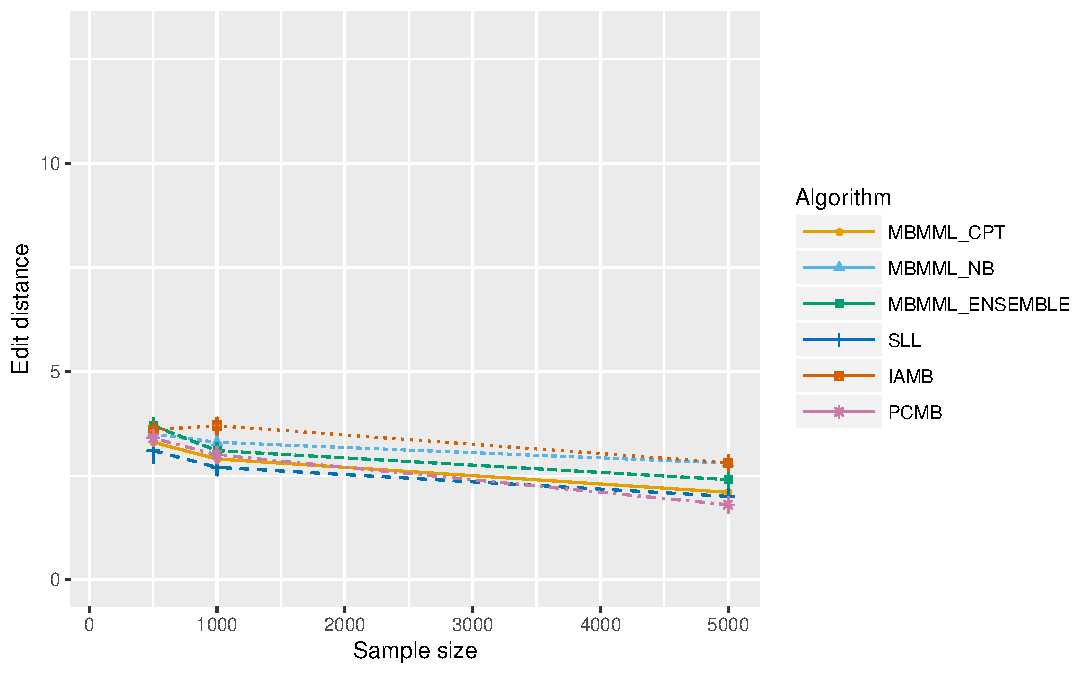
\includegraphics[scale=0.6]{figures/ed_vs_samplesize_insurance.pdf}
  \caption{Edit distance (with $95\%$ confidence intervals) v.s. sample size on INSURANCE network.}
\end{figure}

\begin{figure}[hbt]
  \centering
    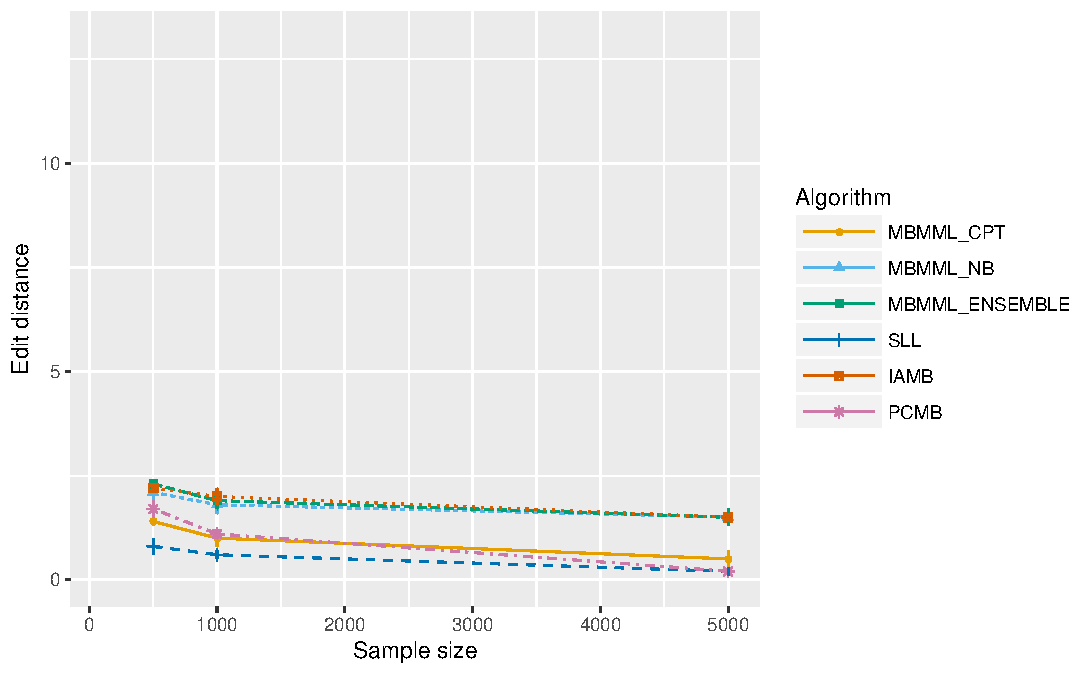
\includegraphics[scale=0.6]{figures/ed_vs_samplesize_alarm.pdf}
  \caption{Edit distance (with $95\%$ confidence intervals) v.s. sample size on ALARM network.}
\end{figure}

\begin{figure}[hbt]
  \centering
    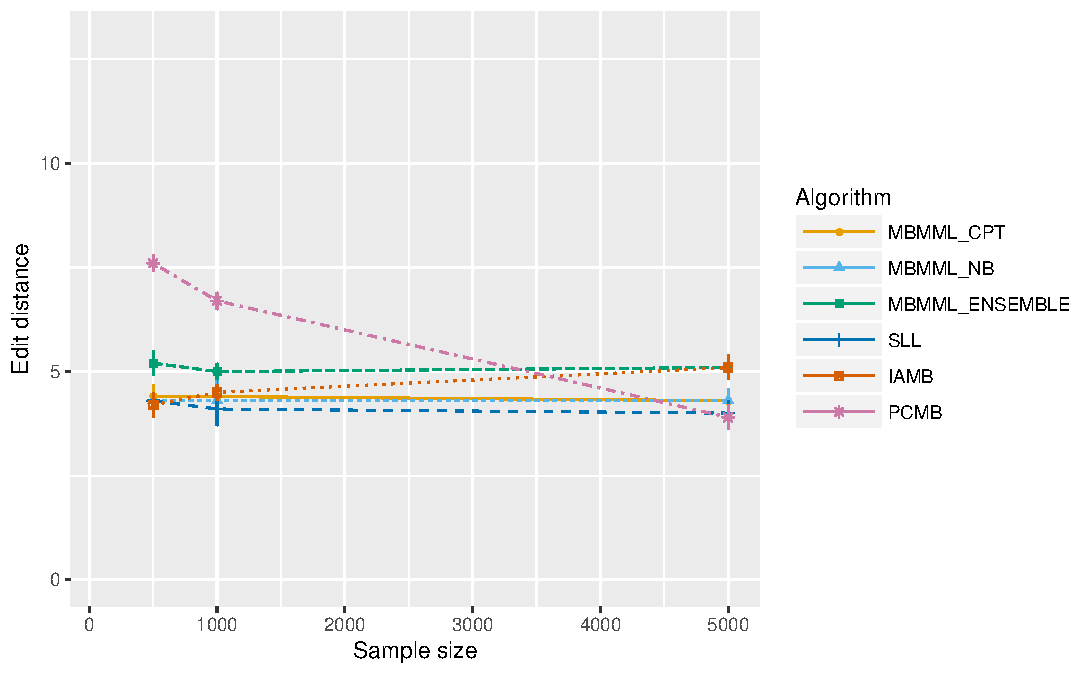
\includegraphics[scale=0.6]{figures/ed_vs_samplesize_hailfinder.pdf}
  \caption{Edit distance (with $95\%$ confidence intervals) v.s. sample size on HAILFINDER network.}
\end{figure}

\begin{figure}[hbt]
  \centering
    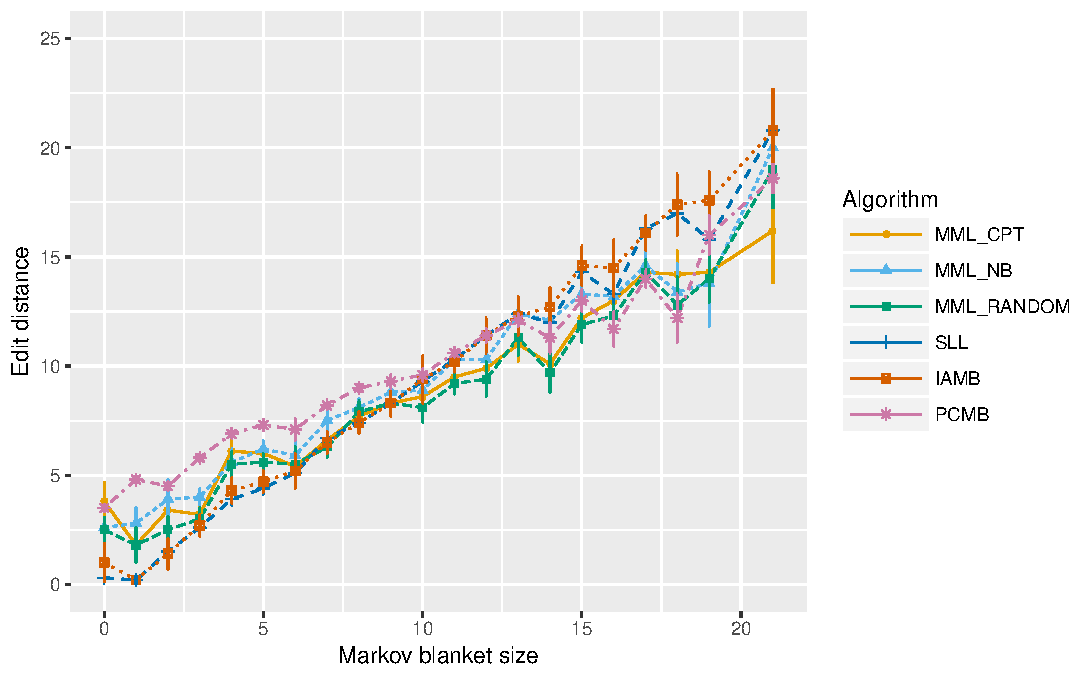
\includegraphics[scale=0.6]{figures/ed_vs_mbsize_30_5_4_1_100.pdf}
  \caption{Edit distance against Markov Blanket size on 30-5-4-1 models with 100 samples.}
\end{figure} 

\begin{figure}[hbt]
  \centering
    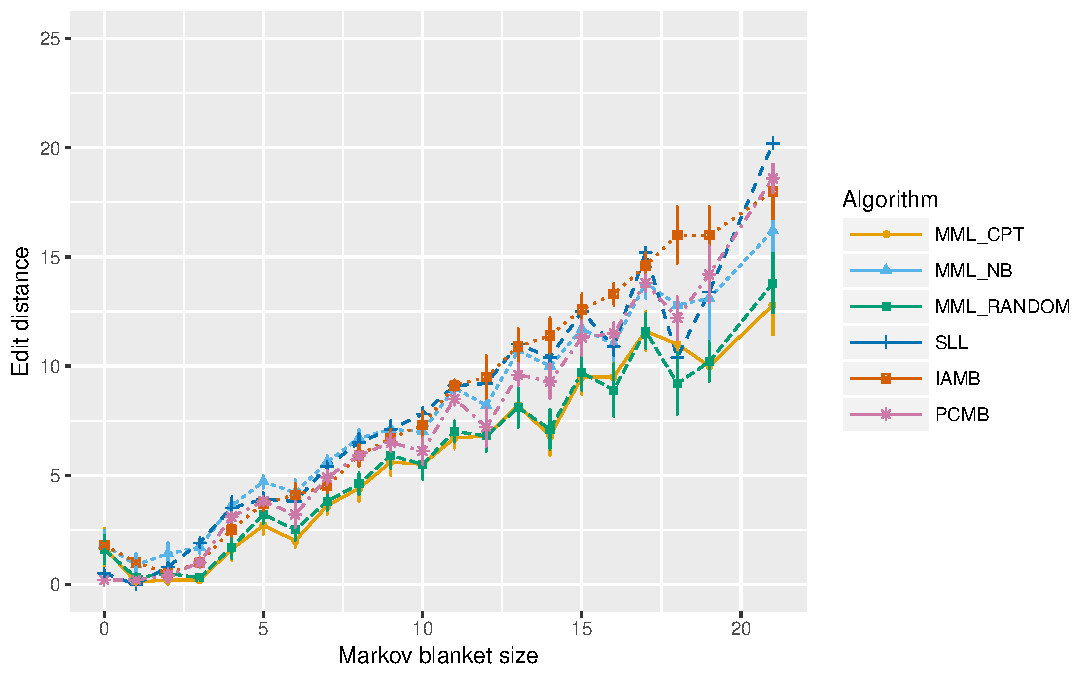
\includegraphics[scale=0.6]{figures/ed_vs_mbsize_30_5_4_1_500.pdf}
  \caption{Edit distance against Markov Blanket size on 30-5-4-1 models with 500 samples.}
\end{figure}

\begin{figure}[hbt]
  \centering
    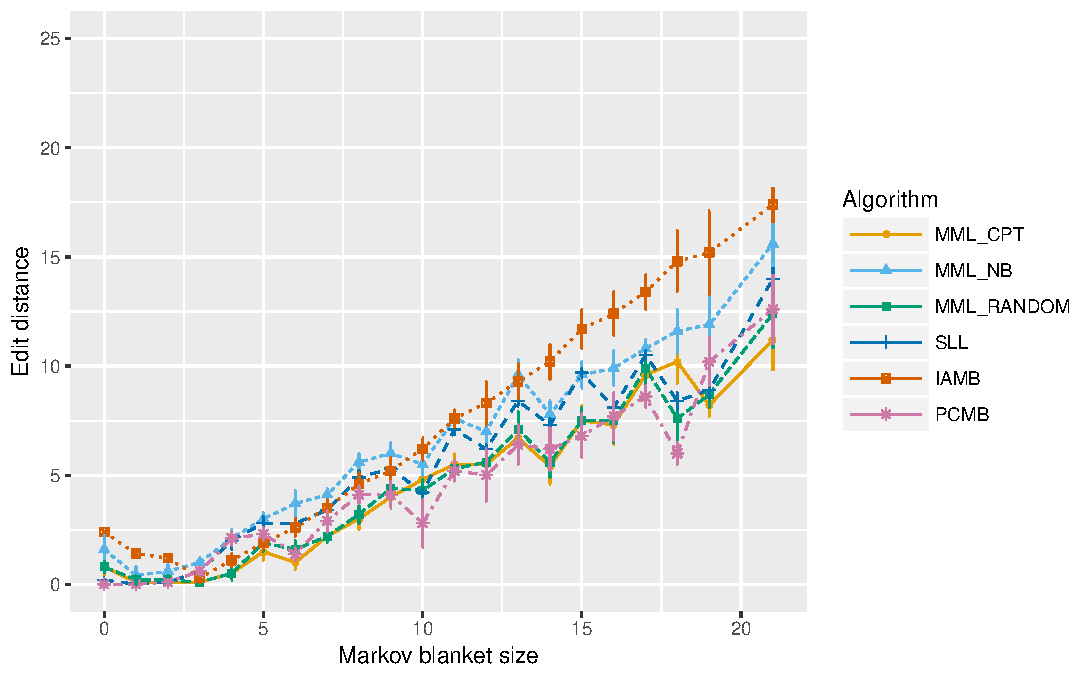
\includegraphics[scale=0.6]{figures/ed_vs_mbsize_30_5_4_1_2000.pdf}
  \caption{Edit distance against Markov Blanket size on 30-5-4-1 models with 2000 samples.}
\end{figure} 

\begin{figure}[hbt]
  \centering
    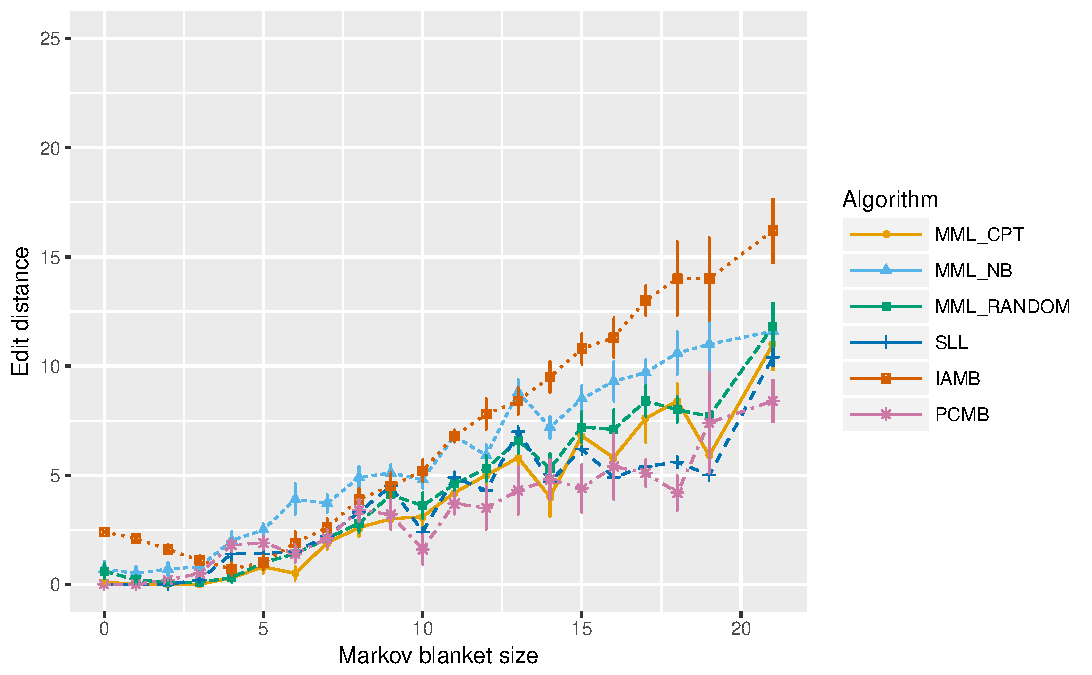
\includegraphics[scale=0.6]{figures/ed_vs_mbsize_30_5_4_1_5000.pdf}
  \caption{Edit distance against Markov Blanket size on 30-5-4-1 models with 5000 samples.}
\end{figure} 

\begin{figure}[hbt]
  \centering
    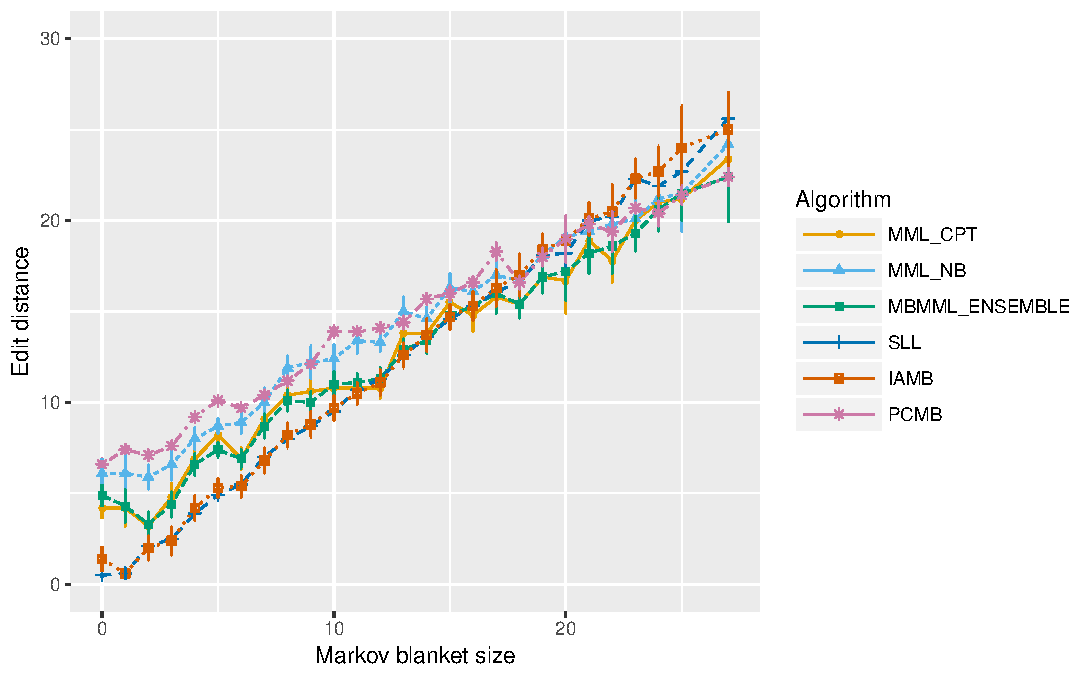
\includegraphics[scale=0.6]{figures/ed_vs_mbsize_50_5_4_1_100.pdf}
  \caption{Edit distance against Markov Blanket size on 50-5-4-1 models with 100 samples.}
\end{figure} 

\begin{figure}[hbt]
  \centering
    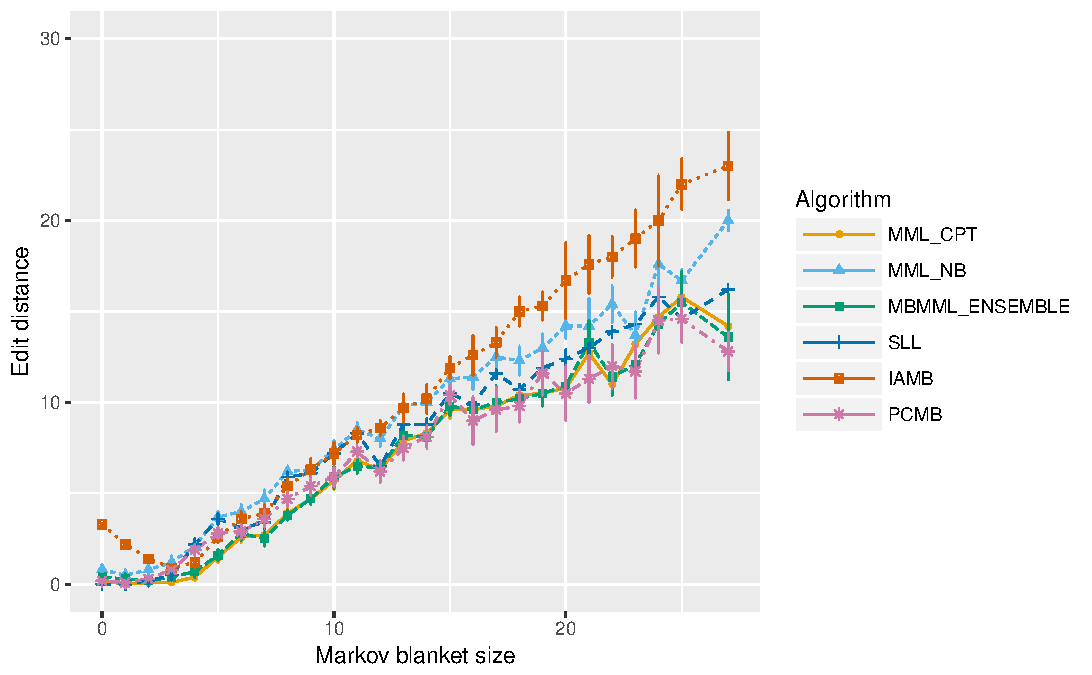
\includegraphics[scale=0.6]{figures/ed_vs_mbsize_50_5_4_1_2000.pdf}
  \caption{Edit distance against Markov Blanket size on 50-5-4-1 models with 2000 samples.}
\end{figure} 

\newpage
\subsection{Notations}
\begin{table}[]
\centering
\caption{Notations}
\label{my-label}
\begin{tabular}{ll}
\hline
$G$ &  a directed acyclic graph\\
$X$ & a variable set \\ 
$E$ & an edge set \\
$P$ & a joint distribution \\
$<G, P>$ & a Bayesian network \\
$\mathcal{H}$ & a model class \\
$H$ & a hypothesis or model \\
$\theta$ &  a set model parameters\\
$\mathcal{D}$ & a set of datasets \\
$D$ & a dataset \\ 
$N$ & the number of observations in a dataset \\
$p(\cdot)$ & the probability of an event \\
$I(\cdot)$ & the information content or message length of an event\\
$|\cdot|$ & the cardinality of a set \\
$X_i$ & the $i^{th}$ variable in $X$ \\ 
$r_i$ & the number of states of a variable $X_i$ \\ 
$\pi_i$ & a parents set of the variable $X_i$ \\ 
$r_{\pi_i}$ & the total number of parents instantiations\\
$\vec{\alpha}$ & a vector of symmetric Dirichlet concentration parameters \\ 
$\alpha_i$ & the $i^{th}$ parameter in $\vec{\alpha}$ \\ 
$n_{ijk}$ & the count of $\pi_i$ is in state $j$ and $X_i$ in state $k$, also known as sufficient statistics\\ 
$n_{ij}$ & the count of $\pi_i$ in state $j$ \\ 
$T_i$ & a Markov Blanket polytree of variable $X_i$ \\
$\mathcal{T}_i$ & a set of Markov Blanket polytrees containing the same set of variables $\{X_i\}\cup MB_i$ \\ \hline
\end{tabular}
\end{table}

%\begin{acknowledgements}
%If you'd like to thank anyone, place your comments here
%and remove the percent signs.
%\end{acknowledgements}

% BibTeX users please use one of
%\bibliographystyle{spbasic}      % basic style, author-year citations
%\bibliographystyle{spmpsci}      % mathematics and physical sciences
%\bibliographystyle{spphys}       % APS-like style for physics
%\bibliography{}   % name your BibTeX data base
\newpage
\bibliographystyle{natbib}
\bibliography{kdd2018}

\end{document}
% end of file template.tex


\documentclass{svmult}

% per springer/quickstart.pdf
\usepackage{mathptmx,helvet,courier,makeidx,graphicx,multicol,footmisc}
\usepackage{amsfonts,ifthen,color}
\usepackage{times,setspace}
%\usepackage{subfig}

\usepackage{latexsym}
\usepackage{graphicx}
\usepackage{amsmath, amssymb, amsfonts, mathtools}
\usepackage{enumerate}
\usepackage{algorithm, algpseudocode}
\usepackage{txfonts, pxfonts}
\usepackage{grffile}
\usepackage{caption, subcaption}
\usepackage{listings}
\usepackage[table, xcdraw]{xcolor}
\usepackage{rotating}
\usepackage{multirow}
\usepackage{chronology}
\usetikzlibrary{arrows, shapes}
\usepackage{tabularx}
\usepackage{hyperref}
\usepackage{libertine}
\usepackage{pgfgantt}
\usepackage{lscape}
\usepackage{setspace} % for double space
\usepackage{enumitem}
%\doublespacing

%\input amssym.def
%\input amssym.tex

\usepackage{natbib,verbatim}
% \usepackage{pdflscape}
%\usepackage{amssymb,latexsym,amsmath}
%\usepackage{graphicx}
\usepackage{url}


\newcommand{\deltap}{\ensuremath{\Delta P}}
\newcommand{\intinf}{\ensuremath{\int_{-\infty}^{\infty}}}
\newcommand{\summ}{\ensuremath{\sum_{i=1}^m}}
\newcommand{\summj}{\ensuremath{\sum_{j=1}^m}}
\newcommand{\ddpi}[1]{\ensuremath{\frac{\delta {#1}}{\delta p_i}}}
\newcommand{\DDpi}[1]{\ensuremath{\frac{\delta^2 {#1}}{\delta p_i^2}}}
\newcommand{\Ddpidpj}[1]{\ensuremath{\frac{\delta^2 {#1}}{\delta p_i \delta p_j}}}

\newcommand{\kl}{\ensuremath{\mathrm{kl}}}
\newcommand{\AL}{\ensuremath{\mathrm{AL}}}
\newcommand{\IR}[1]{\ensuremath{\mathrm{IR}_{#1}}}
\newcommand{\BIR}{\ensuremath{\mathrm{BIR}}}
\newcommand{\IROLD}{\IR{\textit{old}}}
\newcommand{\IRG}{\IR{G}}
\newcommand{\prior}{\ensuremath{\phi}}
\newcommand{\ssec}[1]{\S{}\ref{#1}}

\renewcommand{\cite}{\citep}

\hyphenation{pre-ce-dence Final-ly}

%%%%%%%%%%%%%%%
% 1. Commands
%%%%%%%%%%%%%%%
\newcommand{\dsp}{\setlength{\baselineskip}{24truept}}  %double spacing
\newcommand{\ssp}{\setlength{\baselineskip}{13.6truept}}%single spacing
\newcommand{\hs}{\hspace{0.2in}}
\newcommand{\vs}{\vspace{-0.5in}}
\newcommand{\be}{\begin{equation}}
\newcommand{\ee}{\end{equation}}
\newcommand{\bd}{\begin{description}}
\newcommand{\ed}{\end{description}}
\newcommand{\ben}{\begin{enumerate}}
\newcommand{\een}{\end{enumerate}}
\newcommand{\beq}{\begin{quote}}
\newcommand{\eeq}{\end{quote}}
\newcommand{\bi}{\begin{itemize}}
\newcommand{\ei}{\end{itemize}}
\newcommand{\bea}{\begin{eqnarray}}
\newcommand{\eea}{\end{eqnarray}}
\newcommand{\bua}{\begin{eqnarray*}}
\newcommand{\eua}{\end{eqnarray*}}
\newcommand{\ov}[1]{\overline{#1}}
\newcommand{\ul}[1]{\underline{#1}}
\newcommand{\ba}{\begin{array}}
\newcommand{\ea}{\end{array}}
\newcommand{\bfig}{\begin{figure}}
\newcommand{\efig}{\end{figure}}
\newcommand{\bc}{\begin{center}}
\newcommand{\ec}{\end{center}}
\newcommand{\bt}{\begin{table}}
\newcommand{\et}{\end{table}}
\newcommand{\btab}{\begin{tabular}}
\newcommand{\etab}{\end{tabular}}

\newcommand{\Rarr}{\ensuremath{\Rightarrow}}
\newcommand{\rarr}{\ensuremath{\rightarrow}}
\newcommand{\Larr}{\ensuremath{\Leftarrow}}
\newcommand{\larr}{\ensuremath{\leftarrow}}
\newcommand{\lrarr}{\ensuremath{\leftrightarrow}}
\newcommand{\LRarr}{\ensuremath{\LeftRightArrow}}
\newcommand{\rl}{\ensuremath{\rightleftharpoons}}
\renewcommand{\tilde}{\~{\ }\hspace*{-.7ex}}
\newcommand{\abs}[1]{\ensuremath{~|{#1}|~}}
\newcommand{\seq}[1]{\langle\mbox{#1}\rangle}

\renewcommand{\vec}[1]{\hat{\mathbf{#1}}}  % normal \vec not working

\newcommand{\boxup}[1]
{\beq
\fbox{
\parbox{2in}{#1}}
\eeq
}

\newcommand{\myitem}{\vspace*{-0.5ex} \item }

%\newcounter{modulenum}
%\setcounter{modulenum}{1}
%\newcommand{\module}{% Define module
%\section*{Module \arabic{modulenum}~}
%\addtocounter{modulenum}{1}
%}
%
%\newcounter{problemnum}
%\setcounter{problemnum}{1}
%\newcommand{\problem}{% Define problem
%\subsubsection*{Problem \arabic{problemnum}~}
%\addtocounter{problemnum}{1}
%}
%
%\newcounter{examplenum}
%\setcounter{examplenum}{1}
%\newcommand{\example}{% Define example
%\subsubsection*{Example \arabic{examplenum}~}
%\addtocounter{examplenum}{1}
%}

\newcommand{\mc}[1]{\ensuremath{\mathcal{#1}}}
\newcommand{\optional}[1]{\textcolor{blue}{#1}}
\newcommand{\mmlcpt}{$mbMML_{CPT}$ }
\newcommand{\mbptmml}{$MBPT_{mml}$ }
\DeclareMathOperator*{\argmin}{arg\,min}
\DeclarePairedDelimiter\floor{\lfloor}{\rfloor}
\newcommand{\qedwhite}{\hfill \ensuremath{\Box}}


\newcommand{\indep}{~\raisebox{-0.3ex}{\rotatebox{90}{\ensuremath{\models}}}}
\newcommand{\dep}{\not \hspace*{-1.2ex}\indep}
%\newcommand{\textunder}[1]{$_{\text{#1}}$}

%%%%%%%%%%%%%%%%%%%%%%%%%%%%%%
% 2. Theorems & Environments
%%%%%%%%%%%%%%%%%%%%%%%%%%%%%%

\newtheorem{fact}{Fact}
\newtheorem{hyp}{Hypothesis}
\newtheorem{lemm}{Lemma}
%\newtheorem{exercise}{Exercise}
\newtheorem{Example}{Example}
\newtheorem{prop}{Property}
\newtheorem{defn}{Definition}
\newtheorem{result}{Result}
\newtheorem{conject}{Conjecture}
\newtheorem{princ}{Principle}

%\newenvironment{proof}[1]{{\bf #1}\em}{\/}
\newenvironment{prf}{\rm}{}

  


%%%%%%%%%%
% Misc.
%%%%%%%%%%


%%%%%%%%%%
% Misc.
%%%%%%%%%%

\renewcommand{\floatpagefraction}{0.7}

\newcommand{\cs}[1]{\mbox{c}_{#1}}
\newcommand{\sn}[1]{\mbox{s}_{#1}}
\newcommand{\threevec}[3]{
        \left[ 
        \begin{array}{c} #1 \\ #2 \\ #3 \end{array}
        \right]
}
\newcommand{\hvec}[4]{
        \left[ 
        \begin{array}{c} #1 \\ #2 \\ #3 \\ #4 \end{array}
        \right]
}
\newcommand{\qvec}[1]{
        \left[
        \begin{array}{c} 0 \\ #1 \end{array}
        \right]
}

\newcommand{\newspecial}[1]{
        \ifnum\includefigs>0
                \special{#1}
        \fi
}

\newcommand{\slidehead}[2][2ex]{%
  \slideheading{#2}\vspace{#1}
  \small
  }

\newcommand{\sh}[1]{\slideheading{#1}}

\newcommand{\subheader}[3]{\vspace{#1}\bc{\em #3}\ec\vspace{#2}}

\def\makeslideheading#1{%
  \begin{center}\Large\bf #1\end{center}}

\newboolean{draftp}

\newcommand{\new}[1]{
\textcolor{red}{#1}
}
\newcommand{\newcomment}[1]{
\ifthenelse{\boolean{draftp}}{#1}{}
}


%%%%%%%%%%%%%%%%%%%%
% 3. Page setup
%%%%%%%%%%%%%%%%%%%%


%\setlength{\parindent}{0cm}

\newcommand{\standardpagesetup}{

\addtolength{\textheight}{55mm}
\addtolength{\textwidth}{25mm}
\addtolength{\voffset}{-31mm}
\addtolength{\marginparwidth}{30mm}
%\setlength{\columnsep}{25mm}
%\setlength{\columnseprule}{0.5pt}
\oddsidemargin = 0 mm
\topmargin = 0 mm

%\textwidth = 156 mm
%\textheight = 243 mm
%\parindent = 6 mm
\parskip = 2 mm
\textfloatsep = 0 mm
\intextsep = 0 mm

  }
\newcommand{\pdfpagesetup}{

\addtolength{\textheight}{40mm}
\addtolength{\textwidth}{25mm}
\addtolength{\voffset}{-31mm}
\addtolength{\marginparwidth}{30mm}
%\setlength{\columnsep}{25mm}
%\setlength{\columnseprule}{0.5pt}
\oddsidemargin = 0 mm
\topmargin = 20 mm

%\textwidth = 156 mm
%\textheight = 243 mm
\parindent = 6 mm
%\parskip = 0 mm
\textfloatsep = 0 mm
\intextsep = 0 mm

  }


% afour (a4)
% Hopefully the a4paper option does these, but for reference:
\newcommand{\afour}{
  \paperheight 297mm
  \paperwidth  210mm
  \textheight  247mm % Pageheight - 50mm
  \textwidth   160mm % Pagewidth - 50mm
  \oddsidemargin -5mm
  \topmargin     -15mm
%  \slideheight 152mm % For seminar.sty. As per manual. But use sem-a4.sty.
%  \slidewidth  222mm % Likewise.
  }

% Also try a4 dimensions of 167 and 225 for slideheight/width.


%%%%%%%%%%%%%%%%%%
% 4. Natbib Cites
%%%%%%%%%%%%%%%%%%

%\bibpunct[, ]{(}{)}{,}{a}{,}{,}




% please place your own definitions here and don't use \def but

\makeatletter


% Taken from http://ctan.org/pkg/centernot
\newcommand*{\centernot}{%
  \mathpalette\@centernot
}
\def\@centernot#1#2{%
  \mathrel{%
    \rlap{%
      \settowidth\dimen@{$\m@th#1{#2}$}%
      \kern.5\dimen@
      \settowidth\dimen@{$\m@th#1=$}%
      \kern-.5\dimen@
      $\m@th#1\not$%
    }%
    {#2}%
  }%
}



\makeatother

%
% Insert the name of "your journal" with
% \journalname{myjournal}
%
% This file can be modified and used in other conferences as long
% as credit to the authors and supporting agencies is retained, this notice
% is not changed, and further modification or reuse is not restricted.

\begin{document}
\wow